\chapter{SPECIFICAȚII ȘI REPREZENTAREA APLICAȚIEI}
Aplicația FastRide este construită folosind o arhitectură scalabilă, bazată pe microservicii și servicii în cloud. Tehnologiile principale utilizate sunt Blazor WebAssembly pentru interfața utilizator și Azure Durable Functions pentru logica de backend. Comunicarea dintre cele două componente este realizată prin API-uri HTTP și prin WebSocket-uri cu ajutorul SignalR.

\section{Arhitectura aplicației}
Aplicația dispune de trei nivele:
\begin{itemize}
    \item stocare - unde se păstrează informațiile;
    \item server-side - unde se prelucrează toate infomațiile;
    \item client-side - unde se afișează toate informațiile către utilizatori.
\end{itemize}

\subsection{Stocare}

Azure Table Storage este o bază de date NoSQL, ideală pentru scenarii în care se lucrează cu volume mari de date structurate,
dar fără relații complexe între entități. În cazul aplicației FastRide, fiecare entitate: utilizatori, curse, șoferi online și instanțele de orchestrare, este reprezentată ca o tabelă separată în Table Storage. Fiecare înregistrare (sau entitate) dintr-o tabelă este identificată în mod unic printr-o combinație de \textit{PartitionKey} și \textit{RowKey}, ceea ce asigură o distribuire eficientă și acces rapid la date.
\begin{figure}[H]
    \centering
    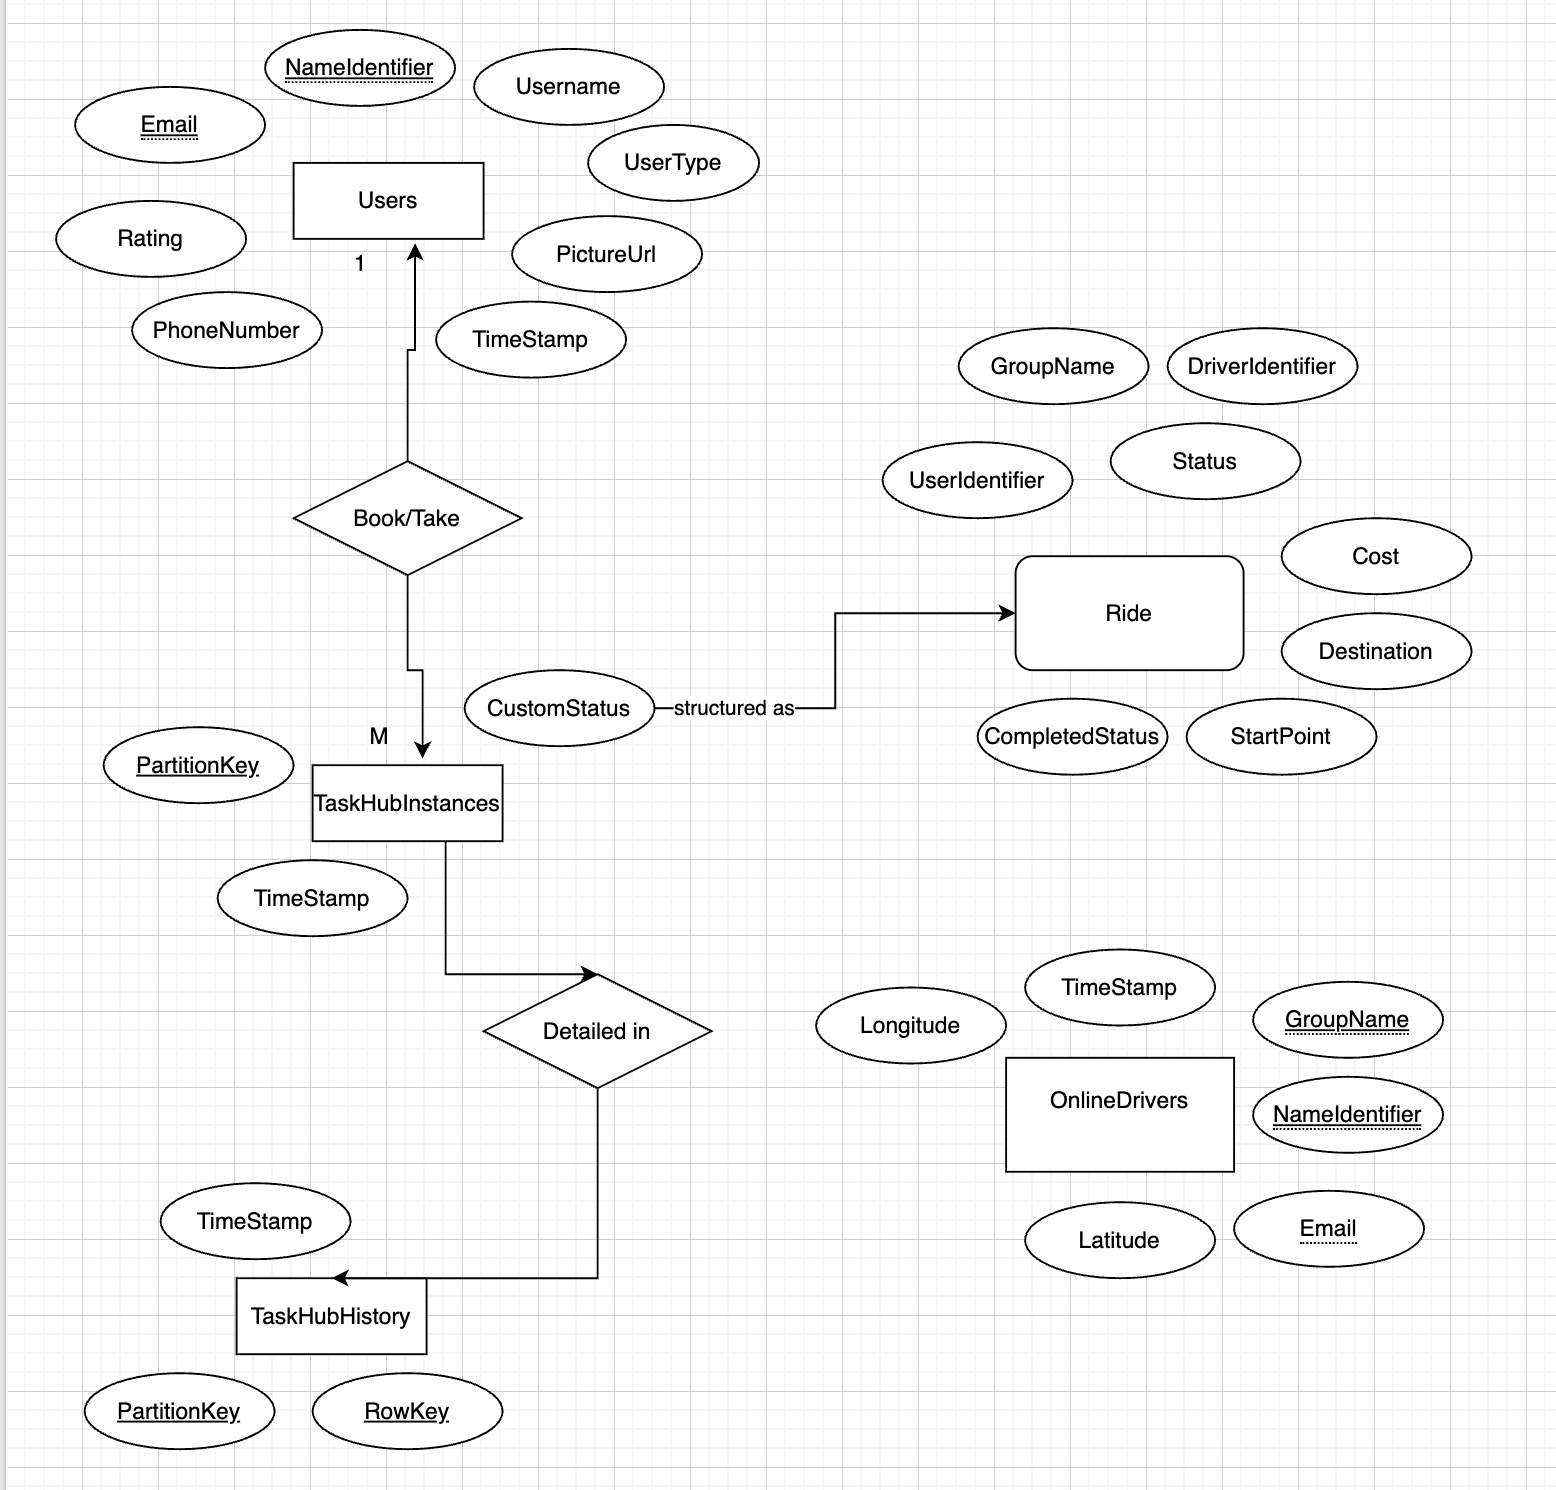
\includegraphics[width=16cm]{Assets/ER.png}
    \caption{Diagrama ER pentru baza de date.}
    \label{fig:ER}
\end{figure}

Aplicația FastRide conține trei entități, fiecare reflectând o componentă critică a funcționalității sistemului: utilizatorii, cursele și șoferii online.

Totul pornește de la entitatea \textit{Users}, care stochează informațiile de bază ale fiecărui utilizator autentificat prin Google.
Fiecare utilizator este identificat în mod unic prin \textit{NameIdentifier} și \textit{Email}, iar alături de acesta se păstrează date precum numele (\textit{Username}), tipul de utilizator (\textit{Driver}, \textit{User} sau \textit{Admin}), ratingul acumulat de-a lungul timpului, numărul de telefon și o eventuală poză de profil (\textit{PictureUrl}).

În momentul în care un utilizator rezervă sau preia o cursă, se creează o relație între acesta și instanțele de orchestrare.
Aici intervin tabelele \textit{TaskHubInstances} și \textit{TaskHubHistory}, care reflectă intern mecanismul
de orchestrare al Azure Durable Functions. Fiecare instanță a unei funcții durabile este stocată în \textit{TaskHubInstances}, iar starea
sa (\textit{CustomStatus}) este utilizată pentru a reflecta progresul unei curse (\textit{Ride}). În paralel, \textit{TaskHubHistory} păstrează detaliile cronologice ale
execuției, istoricul exact al fiecărei acțiuni legate de instanța respectivă. Ambele entități sunt identificate prin \textit{PartitionKey}, iar
în cazul istoricului, și prin \textit{RowKey}.

Starea unei curse este gestionată de modelul \textit{Ride}, care este corelat cu Users prin câmpul \textit{UserIdentifier}, indicând clientul
care a inițiat cererea. Dacă un șofer acceptă cursa, acesta este reprezentat prin \textit{DriverIdentifier}. Fiecare cursă este
caracterizată de un status:
\begin{itemize}
    \item \textit{NewRideAvailable} - status-ul inițial al cursei;
    \item \textit{GoingToUser} - șoferul acceptă cursa și navighează către client;
    \item \textit{GoingToDestination} - șoferul merge spre destinație împreună cu pasagerul;
    \item \textit{Finished} - cursa este finalizată cu success;
    \item \textit{Cancelled} - cursa a fost anulată;
    \item \textit{None} - state-ul inițial.
\end{itemize}
Mereu după ce cursa se termină, aceasta se setează pe state-ul inițial datorită evitării de a complica infrastructura proiectului.
Pentru a face vizibil în continuare statusul final al cursei, aceasta memorează și un \textit{CompletedStatus}:
\begin{itemize}
    \item \textit{DriverNotFound} - nu s-a găsit niciun șofer pentru a finaliza cursa;
    \item \textit{PaymentRefused} - clientul a refuzat plata (disponibilă doar cu cardul);
    \item \textit{Cancelled} - cursa este anulată din orice alte motive;
    \item \textit{Completed} - cursa a fost terminată cu success.
\end{itemize}
În infomațiile cursei se mai regăsesc și punctul de plecare (\textit{StartPoint}),
destinația (\textit{Destination}) și costul asociat. \textit{GroupName} este folosit pentru a lega această entitate de sesiunea real-time
corespunzătoare, utilă pentru actualizări prin SignalR, astfel încât, doar șoferii din același grup cu clientul ce a inițiat cursa pot interacționa.


Pe lângă aceste entități persistente, aplicația păstrează în mod temporar o listă cu șoferii activi prin tabela \textit{OnlineDrivers}.
Fiecare șofer online este identificat prin \textit{NameIdentifier} și asociat cu \textit{GroupName}, astfel încât să poată fi notificat
în timp real dacă există cereri în zona sa. Poziția sa curentă este păstrată prin coordonatele \textit{Latitude} și \textit{Longitude},
permițând localizarea sa pe hartă.

Azure Table Storage oferă performanță, scalabilitate și costuri reduse, iar modelul este suficient
de flexibil pentru a susține dezvoltări ulterioare, cum ar fi introducerea plăților reale, recenziilor textuale
sau programării curselor în avans.

\subsection{Server-side}

Backendul aplicației este construit folosind .NET și Azure Functions, oferind o arhitectură
serverless, scalabilă și eficientă pentru gestionarea întregii logici din spatele aplicației.
Totul pornește de la faptul că aplicația este construită într-un mod în care clientul
(Blazor WebAssembly) comunică prin HTTP și SignalR cu backendul, trimițând cereri sau
ascultând în timp real anumite evenimente.

Structura proiectului Server, este cuprinsă din mai multe niveluri: function triggers, orchestrations,
activities, services și repositories.

\textit{Function triggers} sunt de 3 tipuri: \textit{HttpTrigger}, \textit{TimeTrigger} și \textit{SignalRTrigger}.

\textit{HttpTriggers} sunt folosite pentru comunicarea cu Client-side, și sunt requesturi de tipul \textit{Get}/\textit{Post} și \textit{Put}.
\begin{figure}[H]
    \centering
    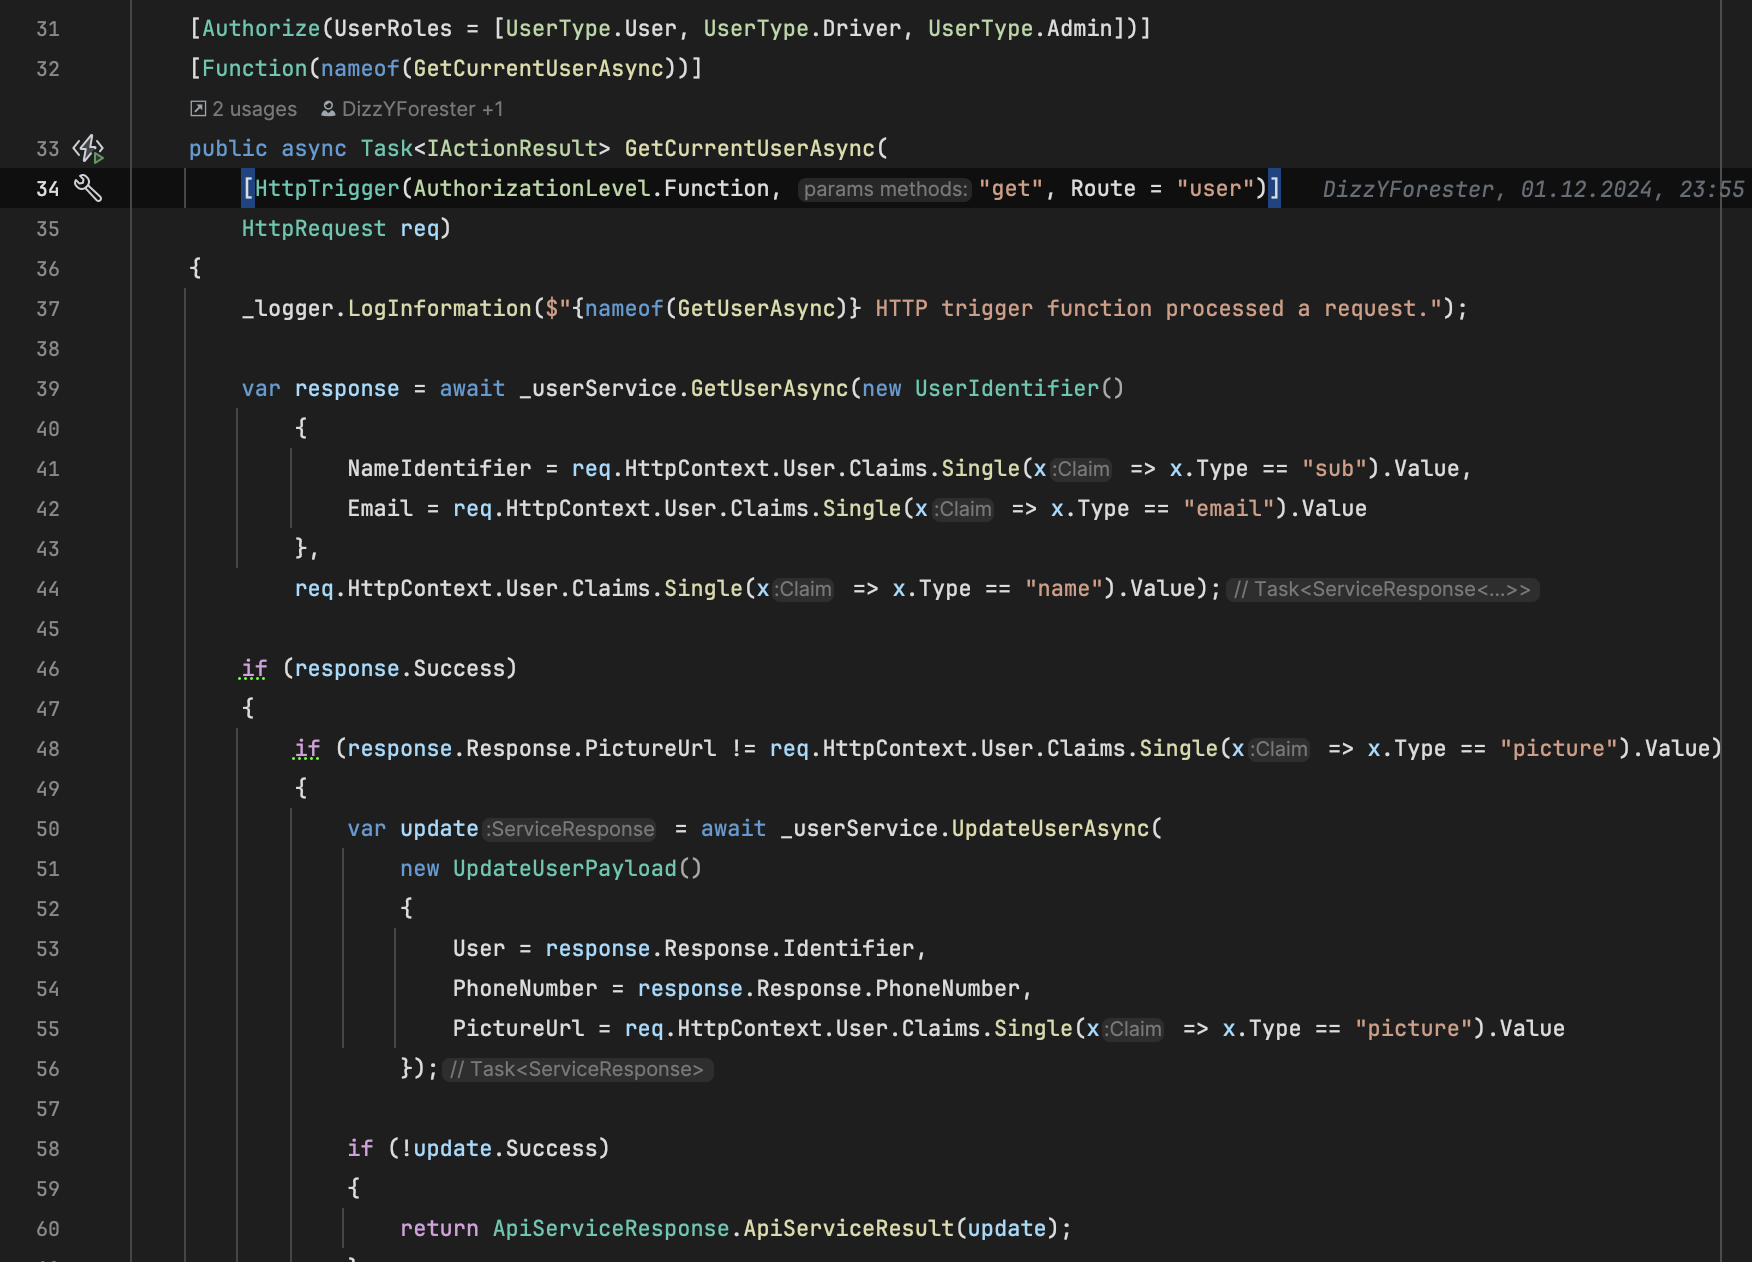
\includegraphics[width=16cm]{Assets/HttpTrigger.png}
    \caption{Exemplu de metodă GET pentru HttpTrigger function.}
    \label{fig:HttpTrigger}
\end{figure}

Aceste request-uri sunt autorizate prin JWT token obținut de la Google. Astfel s-a creat un atribut custom,
ce poate fi folosit doar pe metode, unde se pot defini o listă de \textit{roles} ce pot
accesa metoda respectivă.
Ca și request, body-ul este încapsulat în modelul \textit{HttpRequest} și poate fi deserializat
astfel:
\begin{figure}[H]
    \centering
    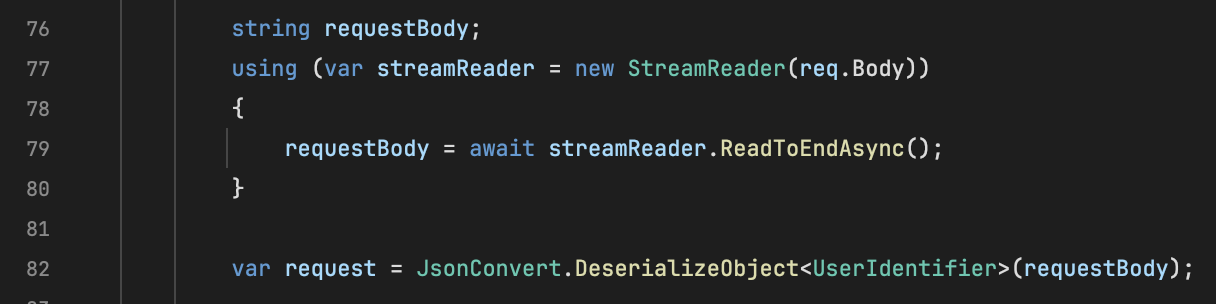
\includegraphics[width=14cm]{Assets/DeserializeRequest.png}
    \caption{Deserializarea unui request într-un tip concret (ex: \textit{UserIdentifier}).}
    \label{fig:DeserializeRequest}
\end{figure}

Ca și răspuns, toate funcțiile HTTP întorc un \textit{IActionResult} ce este mapat printr-o extensie
a unui \textit{ServiceResponse}. Acest model conține status-ul request-ului, mesajul de eroare (dacă
există) și payload-ul response-ului. Toate service-urile returnează un \textit{ServiceResponse}
care, la fel, conține payload-ul, dacă este cu succes sau nu și mesajul de eroare împreună cu excepții.
Dacă există mesaj de eroare atunci rezultatul este un \textit{Bad Request (400)}, iar dacă există
excepție atunci se traduce ca \textit{Internal Server Error (500)}.

\begin{figure}[H]
    \centering
    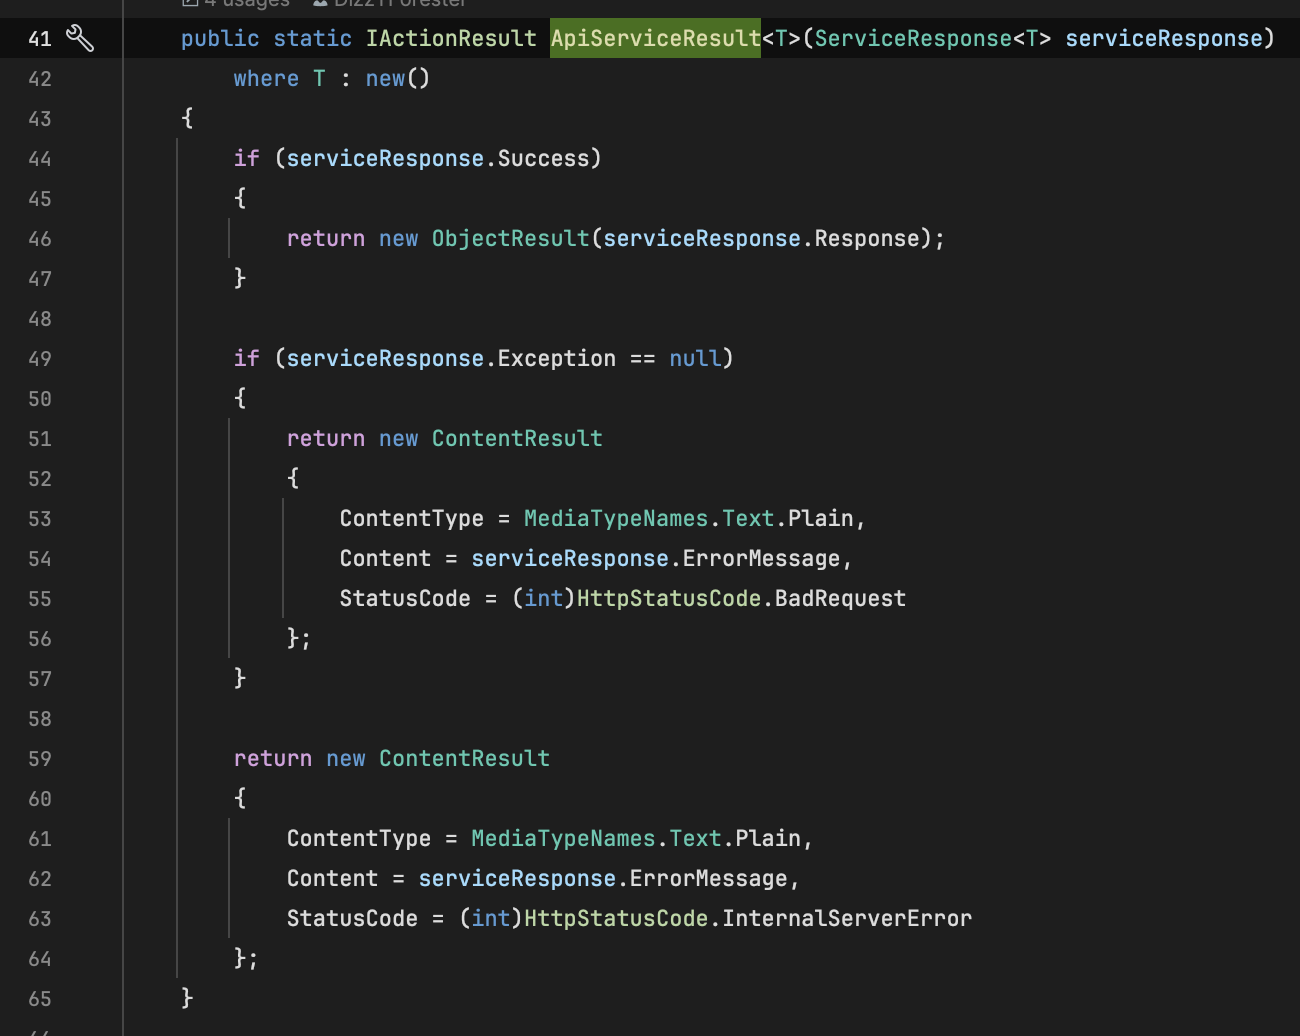
\includegraphics[width=14cm]{Assets/HttpResponse.png}
    \caption{Maparea unui \textit{ServiceResponse} la \textit{IActionResult}.}
    \label{fig:HttpResponse}
\end{figure}

Metodele HTTP disponibile pentru Client sunt:
\begin{itemize}
    \item \textit{GetCurrentUserAsync} pentru a lua informațiile despre user-ul de a inițiat requestul;
    \item \textit{GetUserAsync} pentru a lua informațiile despre un user;
    \item \textit{GetUsers}, disponibil doar pentru admini, pentru a vedea toți utilizatorii;
    \item \textit{UpdateUserAsync} pentru a actualiza un user;
    \item \textit{GetRidesByUserAsync} pentru a afișa cursele unui utilizator
\end{itemize}

Pentru a autoriza aceste endpoint-uri, în Azure Functions se pot înregistra \textit{middleware} pentru
a verifica token-ul. Astfel \textit{AuthenticationMiddleware} și \textit{AuthorizationMiddleware} se ocupă de autentificarea
și autorizarea API-ului, luând JWT token-ul din \textit{Authorization} header, și îl validează
folosind API-ul de la Google.

\begin{figure}[H]
    \centering
    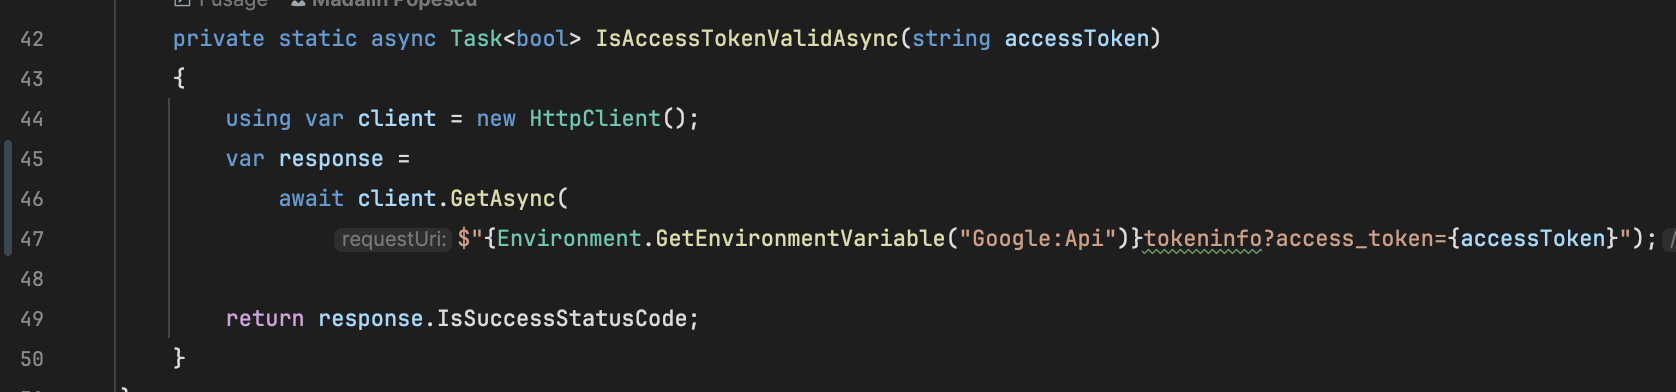
\includegraphics[width=16cm]{Assets/GoogleAuthorization.png}
    \caption{Verificare \textit{AccessToken} folosind Google API.}
    \label{fig:GoogleAuthorization}
\end{figure}

Pentru a face Google API conștient despre existența aplicației și token-ului pe care user-ul îl obține
prin autentificarea pe Client, în Google Console, se creează un \textit{Credential} pentru proiect.
Redirect URIs și request browser sunt reprezentate de Client URL (de acolo se apelează autentificarea).

\begin{figure}[H]
    \centering
    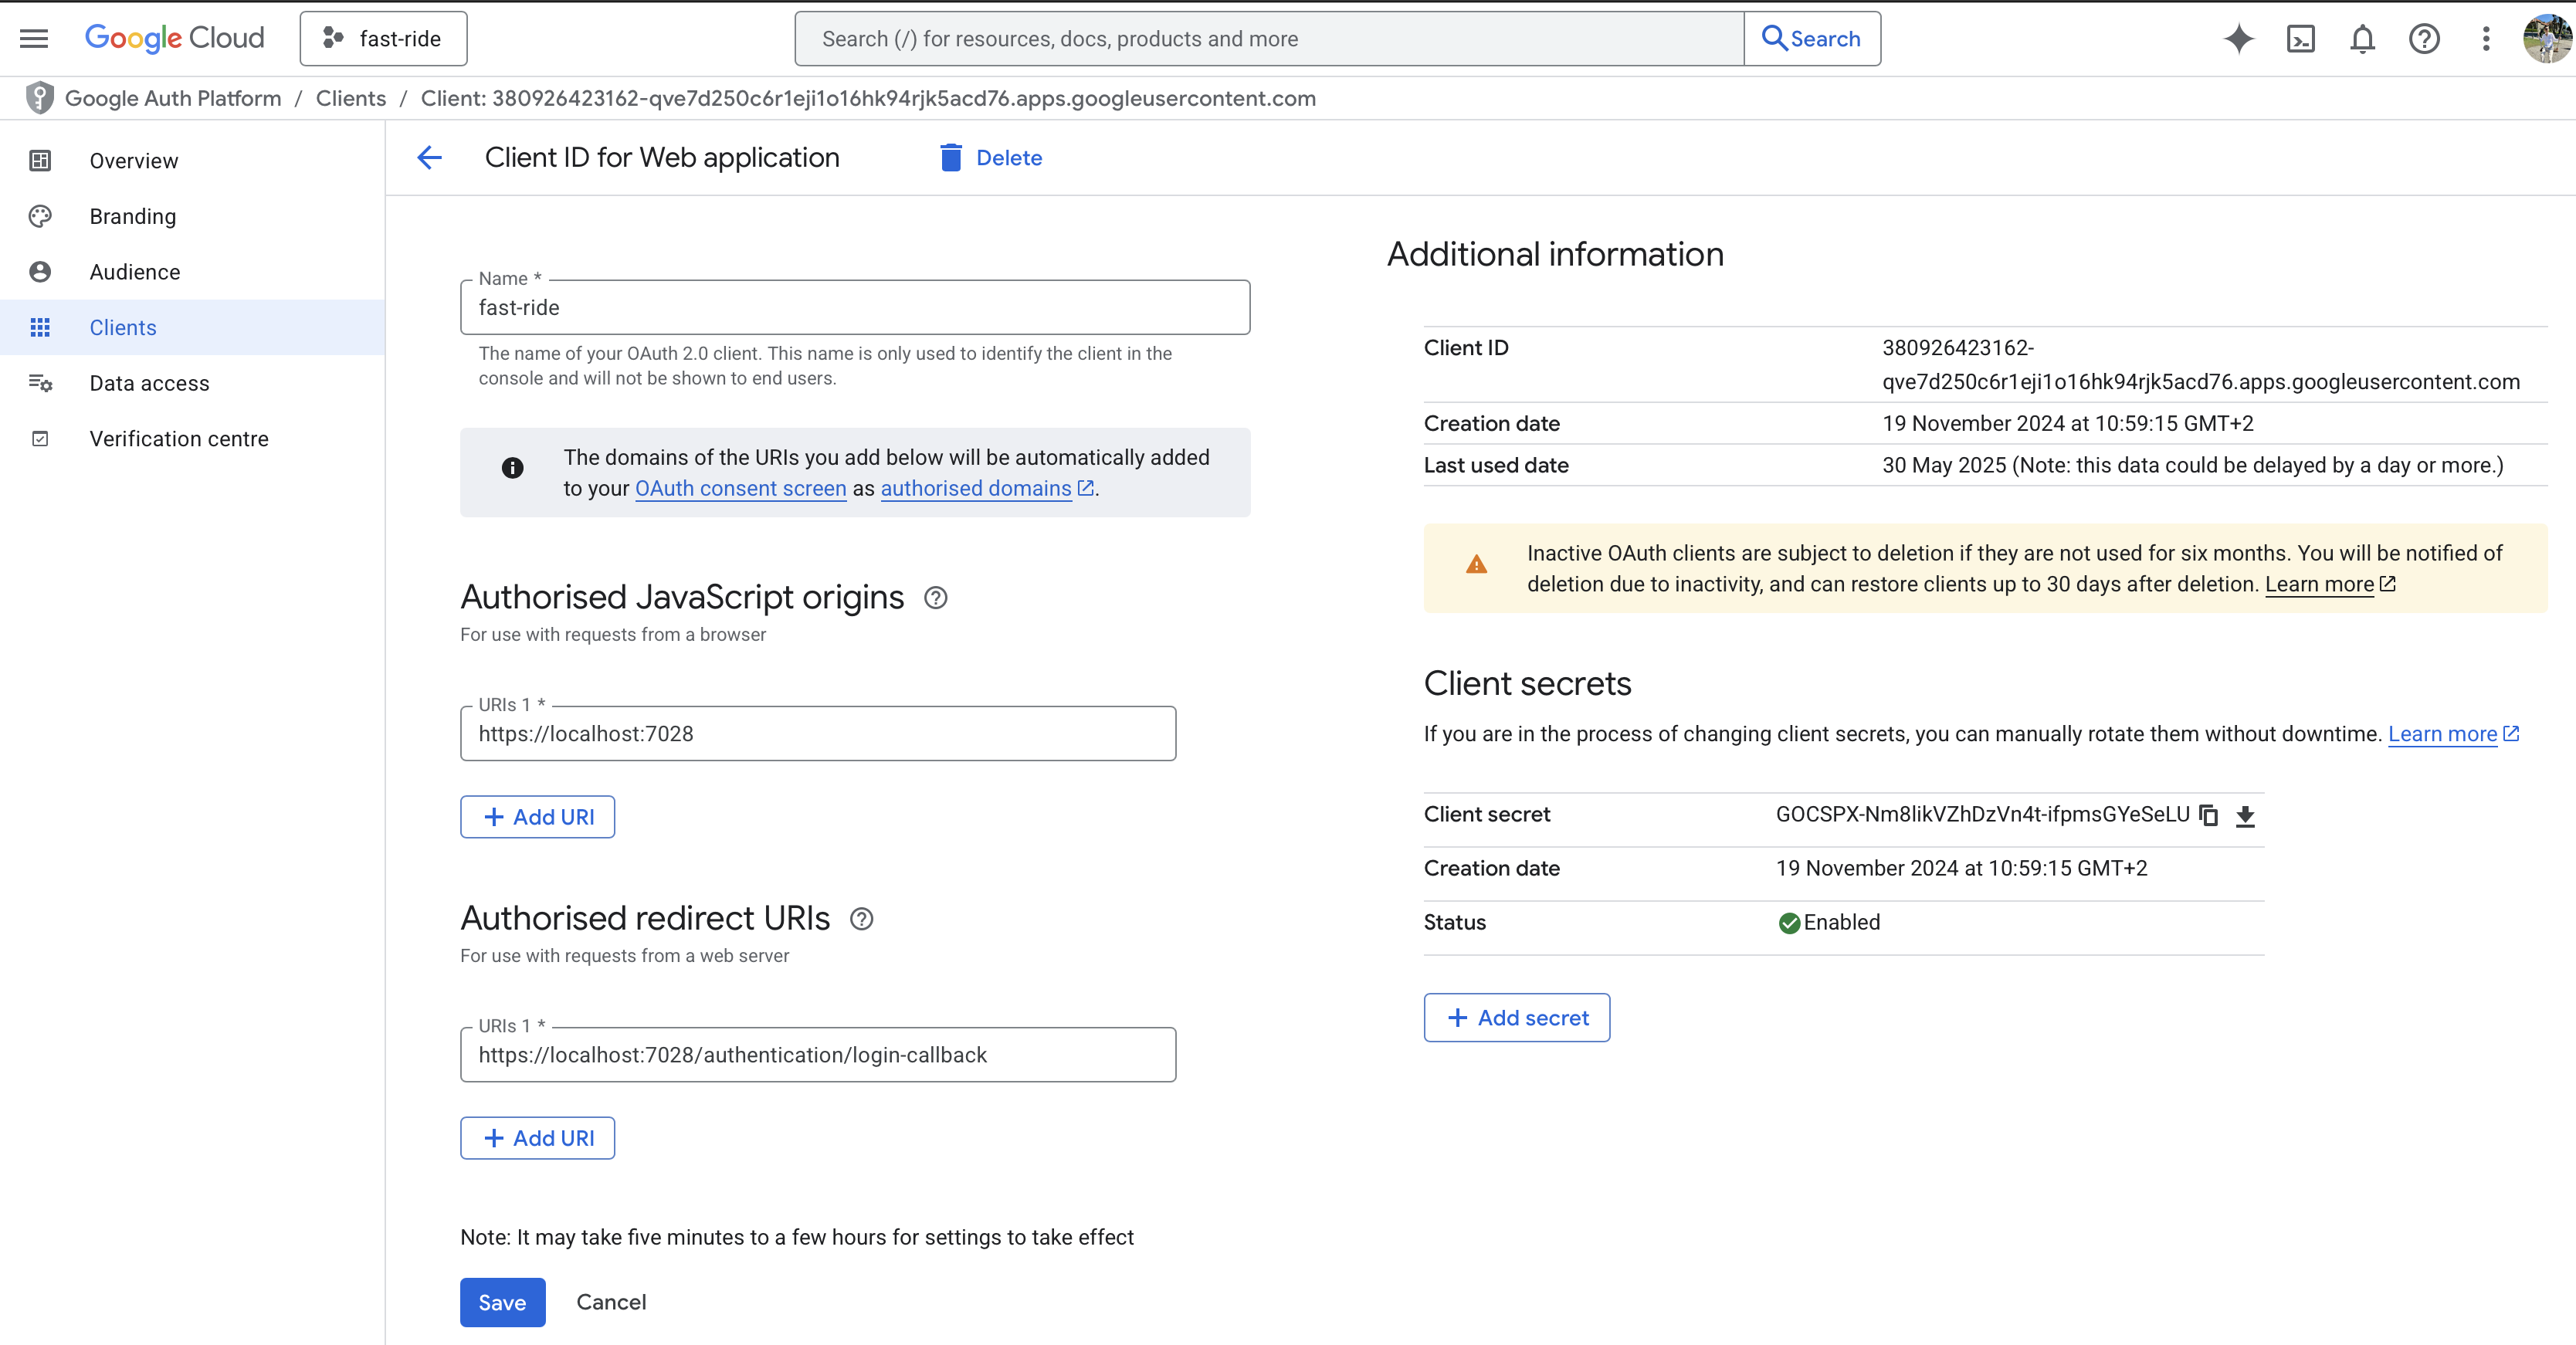
\includegraphics[width=14cm]{Assets/GoogleConfig.png}
    \caption{Configurația Google Credentials.}
    \label{fig:GoogleConfig}
\end{figure}

\textit{TimeTrigger} functions reprezintă funcțiile ce se auto-apelează la o perioadă de timp configurată.
FastRide folosește un acest tip de funcție pentru a interoga din 5 în 5 secunde tabelul generat
de Durable Orchestation în scopul de a găsi curse ce se află în progres și de a le notifica
Client-ului prin SignalR.

\begin{figure}[H]
    \centering
    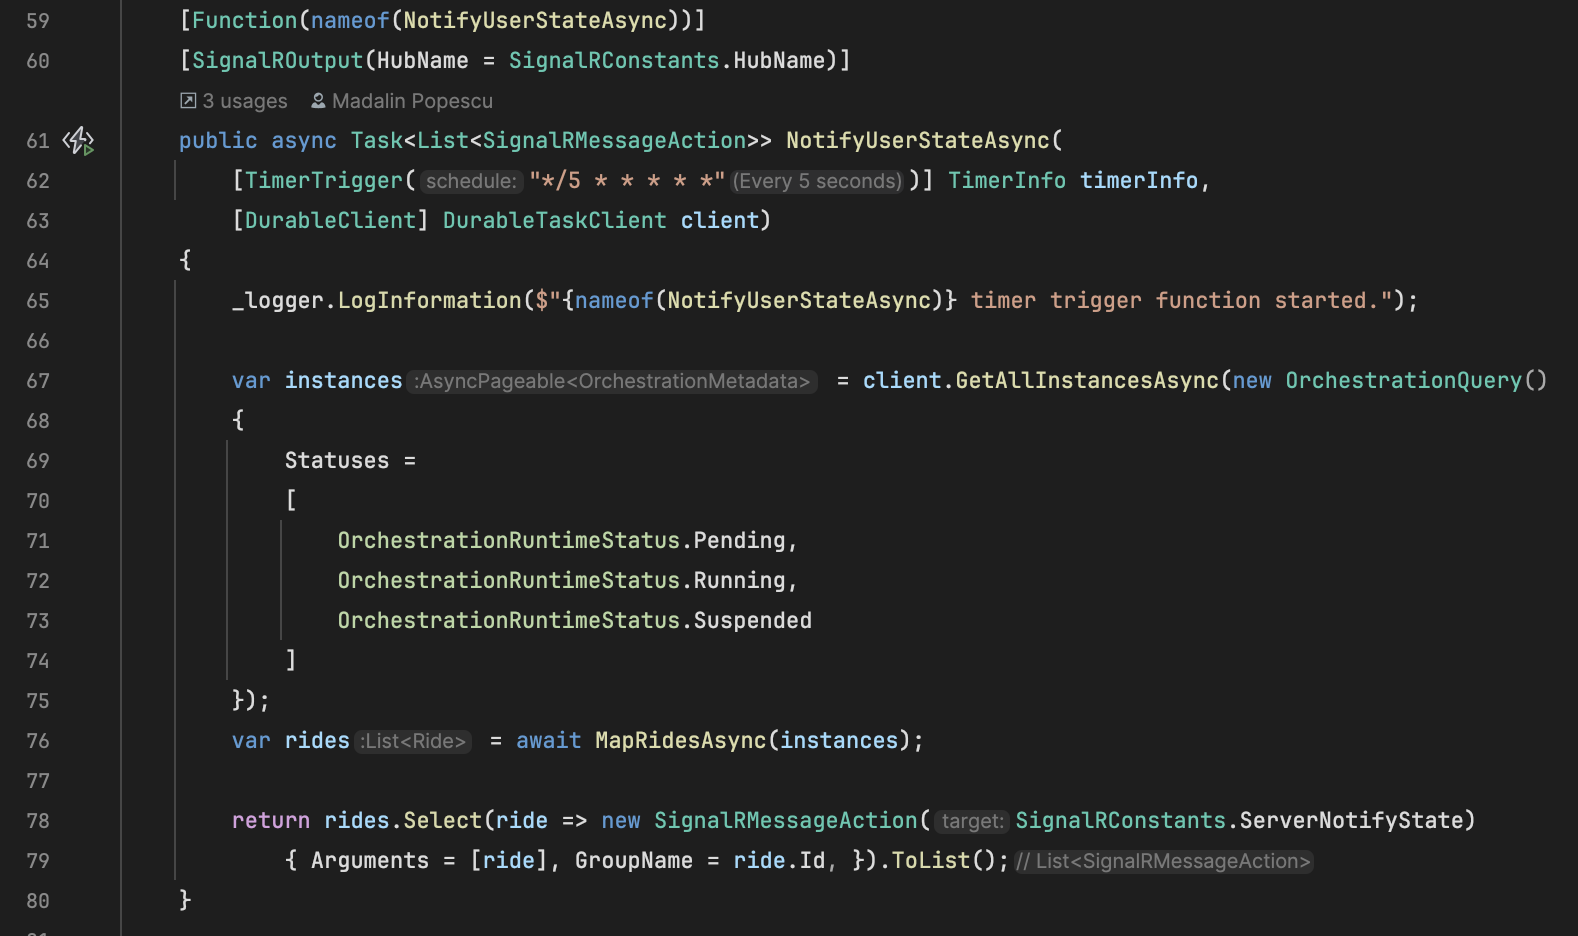
\includegraphics[width=16cm]{Assets/TimeTrigger.png}
    \caption{TimeTrigger function ce interoghează Durable tables și notifică utilizatorii despre curse lor ce sunt în desfășurare.}
    \label{fig:TimeTrigger}
\end{figure}
Această funcție caută orchestrările ce se află în \textit{Pending}, \textit{Running} sau \textit{Suspended},
citește proprietatea \textit{CustomStatus} unde se regăsesc informațiile complete ale cursei și
le returnează pentru fiecare grup de utilizatori ce se află în parcursul cursei respective (în acest caz, \textit{GroupName} devine \textit{ride.Id} - ID-ul cursei).

\textit{SignalRTrigger} sunt function-urile ce ascultă la un canal WebSocket pentru SignalR, dar sunt și capabile să returneze
un mesaj către acest canal. Acestea sunt folosite pentru comunicarea în timp real cu Client-ul și au rolul de a notifica
utilizatorii despre diferite acțiuni ce trebuie să le facă (ex: să plătească, să accepte o cursă, etc).
Acest tip de funcții folosesc un \textit{eventType} ca și identificator pentru a notxifica utilizatorii ce sunt
conectați la canal. Utilizatorii pot fi grupați în grupuri pentru a trimite mesaje doar către un
anumit grup, însă se pot trimite mesaje și direct către un utilizator specific.

FastRide folosește grupurile pentru a grupa utilizatorii per orașe, astfel cei din Craiova nu pot
vedea și nu pot primi sau trimite mesaje de la sau către cei din București, spre exemplu. Grupurile se mai folosesc și
pentru a identifica doi utilizatori ce se află într-o cursă, astfel în momentul în care o cursă se inițiază,
atât șoferul cât și clientul, părăsesc automat grupul din care fac parte (o combinație dintre țară, județ și oraș)
și se înscriu la grupul ce se formează din ID-ul cursei generat la creare.

Pentru a se conecta la canalul de SignalR și pentru a se înscrie într-un grup sau pentru
a părăsi un grup, Client-ul trebui sa apeleze câteva metode care indică aceste \textit{actions}.

\begin{figure}[H]
    \centering
    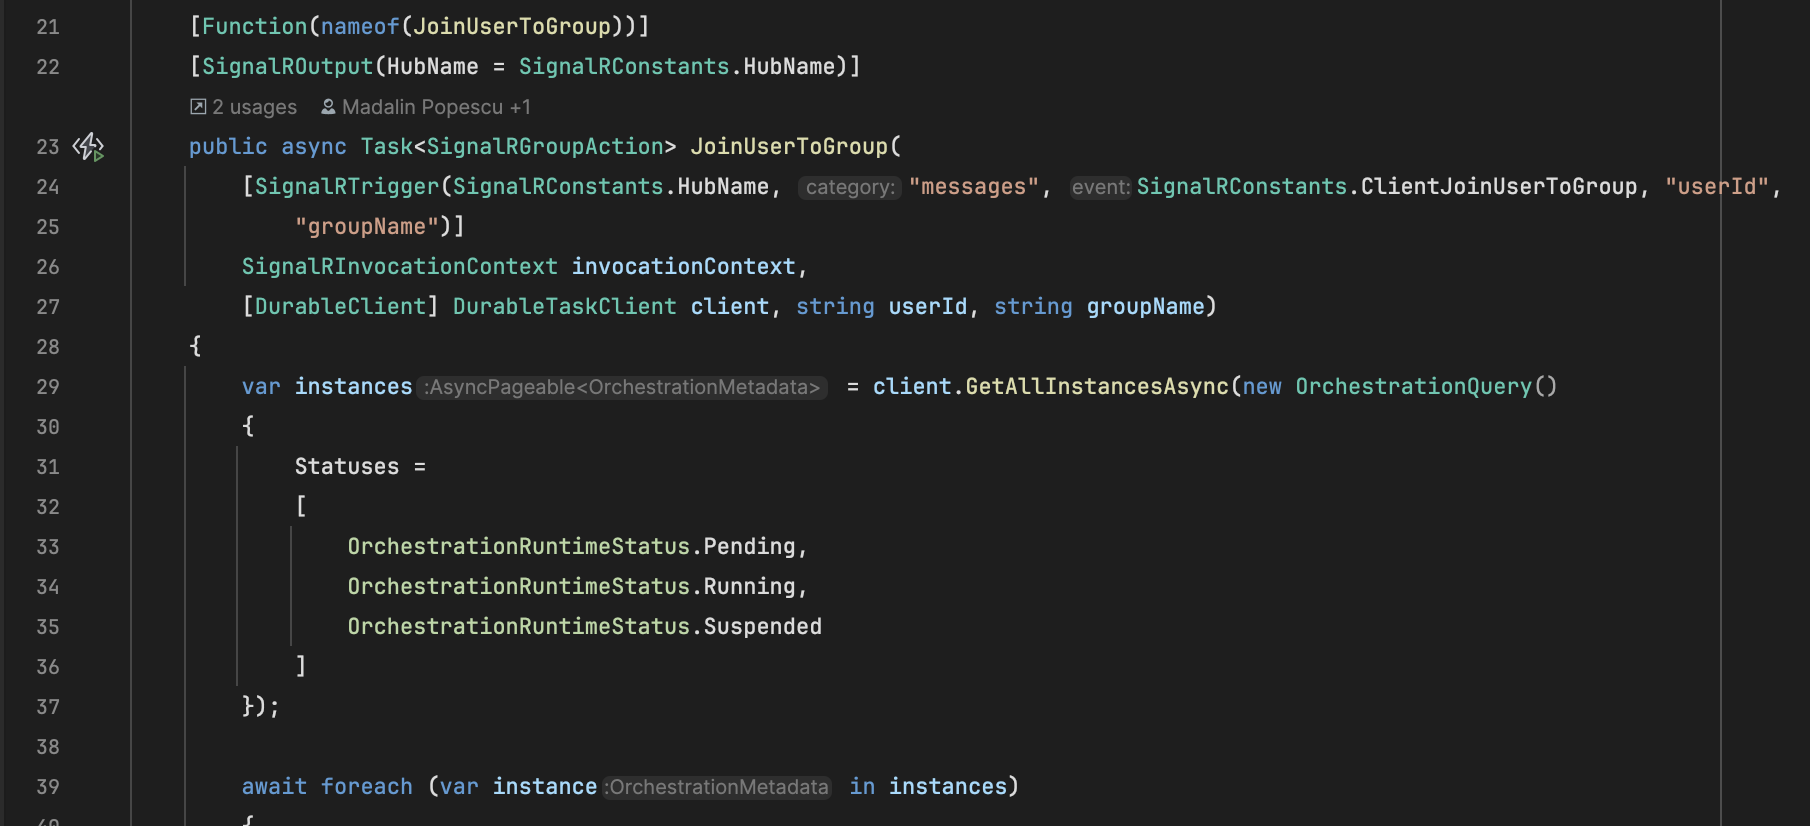
\includegraphics[width=16cm]{Assets/JoinUser.png}
    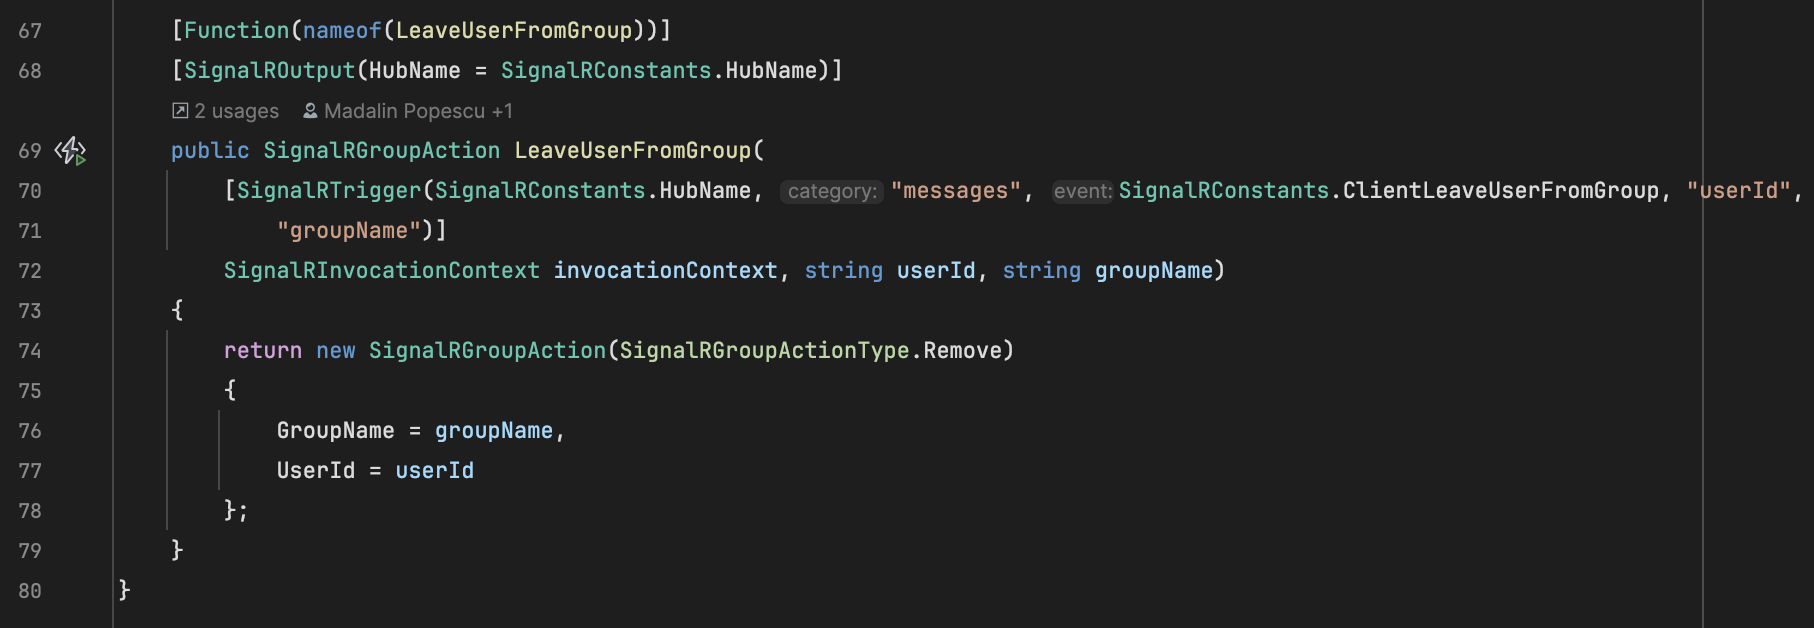
\includegraphics[width=16cm]{Assets/RemoveUser.png}
    \caption{Înscrierea și ștergerea unui utilizator din grup.}
    \label{fig:JoinRemoveUser}
\end{figure}

Pentru ca server-ul SignalR să înregistreze acțiunile aferente, Server-ul
trebuie să returneze un \textit{SignalRGroupAction}. Pentru restul notificările
se folosește \textit{SignalRMessageAction}.

Conectarea la SignalR de către utilizator și notificarea că a fost conectat sau
deconectat cu succes se face prin metodele din imaginile din fig. \ref{fig:negotiateConnectDisconnect}.
Astfel, în momentul în care un șofer este conectat sau deconectat, se poate actualiza
tabela \textit{OnlineDrivers}.

Se observă faptul că este nevoie de un identificator al utilizatorului, acesta fiind \textit{NameIdentifier}-ul
din storage, care este totodată și claim-ul \textit{sub} din JWT token-ul de la Google, doar că hash-uit (SHA256).
Hash-ul se aplică pentru a obține o structură de \textit{GUID}.

\begin{figure}[H]
    \centering
    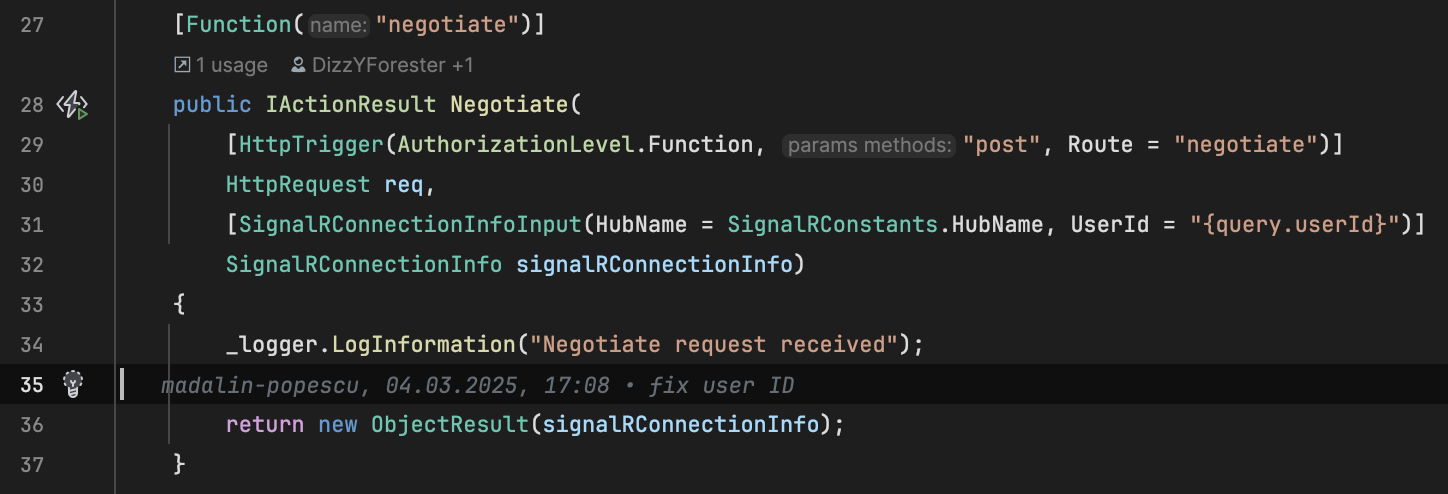
\includegraphics[width=16cm]{Assets/negotiate.png}
    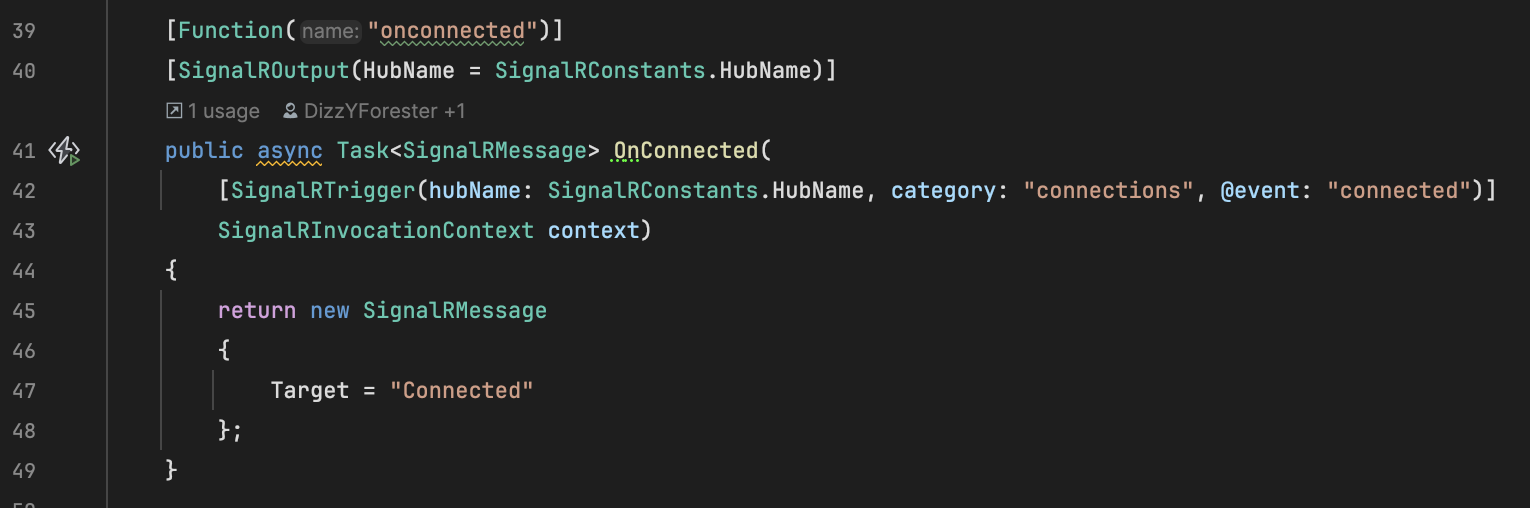
\includegraphics[width=16cm]{Assets/onconnected.png}
    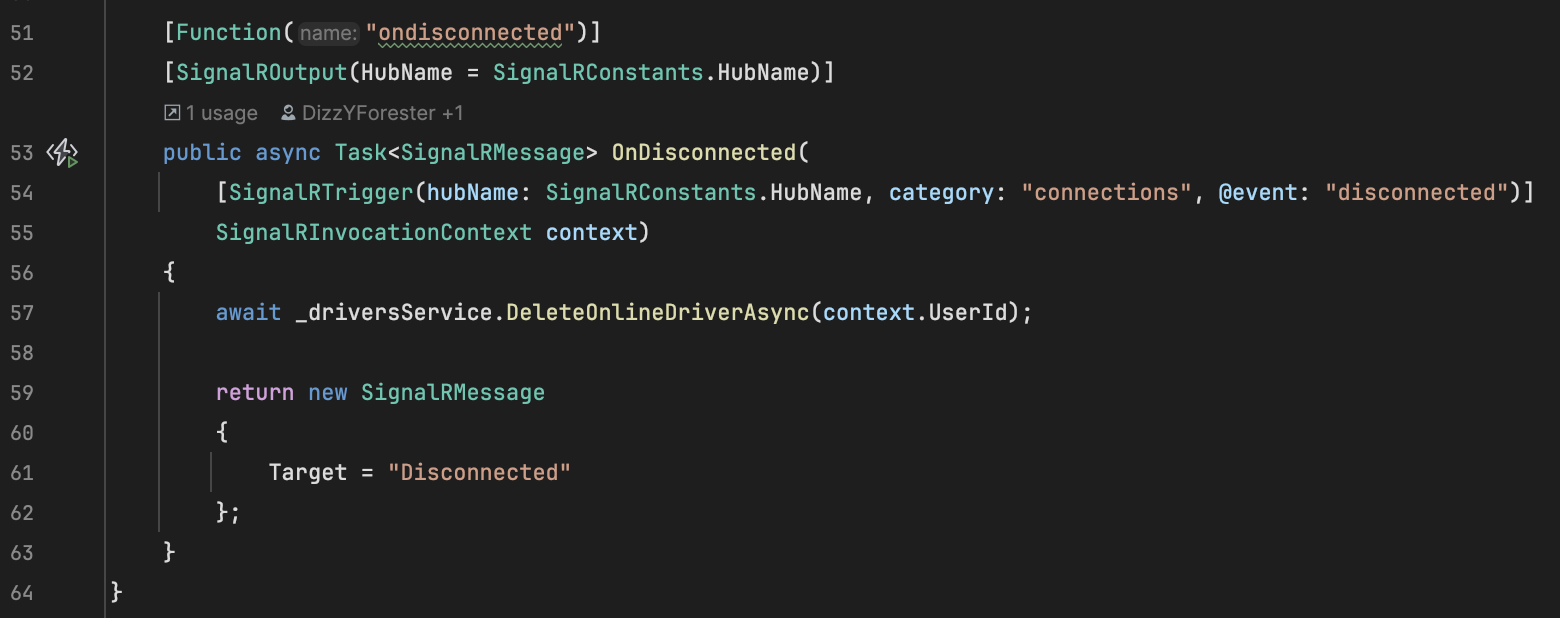
\includegraphics[width=16cm]{Assets/ondisconnected.png}
    \caption{\textit{Negotiate}, conectarea și deconectarea unui utilizator de la conexiune SignalR.}
    \label{fig:negotiateConnectDisconnect}
\end{figure}

\textit{Orchestrations} sunt Azure Functions ce pot rula mai mult de 5 minute, ce își păstrează
state-ul în tabele, astfel încât indiferent de ce se întâmplă cu runtime-ul aplicației,
acestea își continuă execuția fără a relua tot procesul.

În proiect, există o singură funcție de acest gen, ce se ocupă cu flow management-ul unei curse.
Astfel, ea primește ca și input, un request ce conține un \textit{User} (clientul), locul de unde se inițiază
cursa și destinația dorită. La fiecare pas, aceste infomații se actualizează și
se salvează în coloana specială a Durable Orchestrations, \textit{CustomStatus}, totodată, modificând și status-ul
cursei.

\begin{figure}[H]
    \centering
    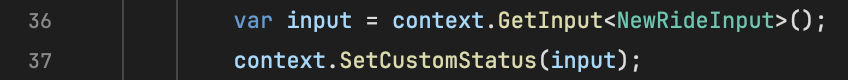
\includegraphics[width=14cm]{Assets/saveCustomStatus.png}
    \caption{Salvarea în \textit{CustomStatus} a request-ului inițial.}
    \label{fig:saveCustomStatus}
\end{figure}

Mai departe, aplicația calculează prețul cursei și trimite către utilizator un request de confirmare a cursei.
Pentru a aștepta răspuns, Durable Orchestrations folosesc evenimente pe care le așteaptă:
\begin{figure}[H]
    \centering
    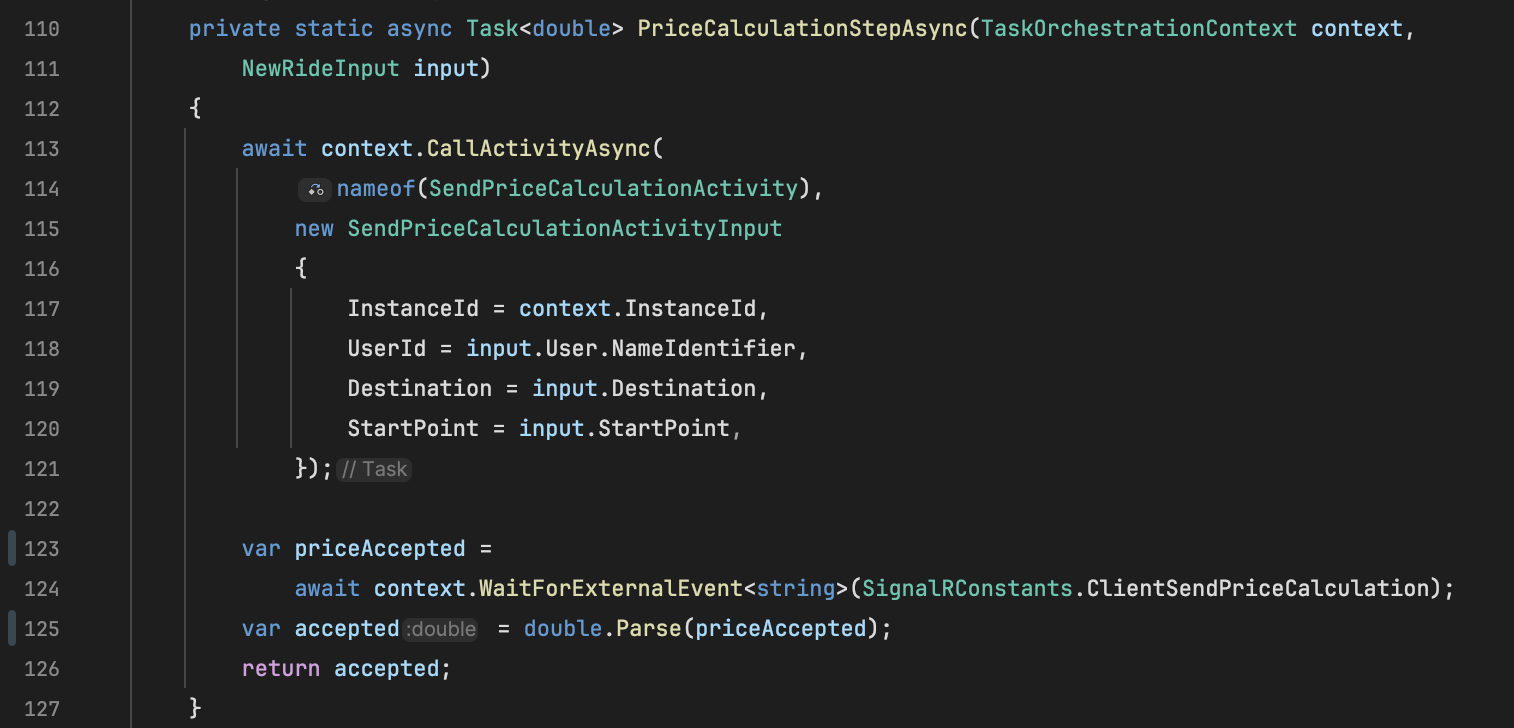
\includegraphics[width=16cm]{Assets/waitForEvent.png}
    \caption{Trimiterea confimării către utilizator și așteptarea răspunsului.}
    \label{fig:waitForEvent}
\end{figure}
Pentru a calcula prețul se folosește următoarea formulă (distanța dintre 2 puncte în spațiu, estimarea timpului de
parcurgere cu un timp comun și prețul configurat pentru fiecare kilometru și minut, totul adunat cu o sumă inițială):
\begin{figure}[H]
    \centering
    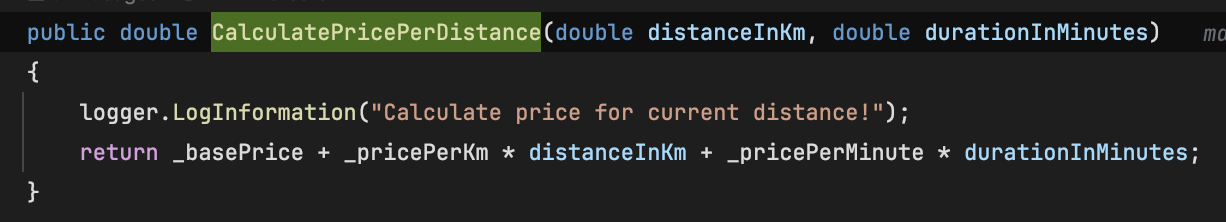
\includegraphics[width=15cm]{Assets/calculatePrice.png}
    \caption{Calcularea prețului cursei.}
    \label{fig:calculatePrice}
\end{figure}
Dacă s-a acceptat, urmează să se inițieze plata, astfel, Server-ul se ocupă cu creearea
unui \textit{PaymentIntent} ce se poate folosi pentru a se realiza plata cu succes. Fără acestă intenționare,
Stripe nu știe să autentifice request-ul de plată.
\begin{figure}[H]
    \centering
    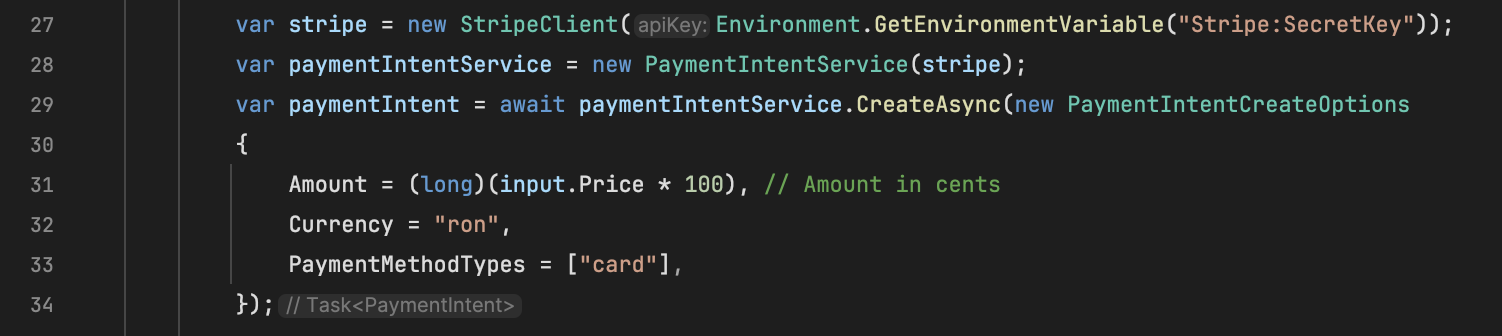
\includegraphics[width=16cm]{Assets/intent.png}
    \caption{Crearea \textit{PaymentIntent}-utului prin Stripe.}
    \label{fig:intent}
\end{figure}
Mai departe, după ce plata s-a procesat cu success, începe să se caute un șofer pentru cursă.
Algoritmul de căutare se folosește de tabelul \textit{OnlineDrivers} pentru a identifica poziția
fiecărui șofer și a îi calcula distanța de la client la acesta. Șoferii se iau în ordine până se găsește
unul sau niciunul. Dacă șoferul nu acceptă cursa în timp de 35 secunde, se consideră ca și respinsă.
Pentru a face acest lucru posbil, se creează o listă de \textit{Task}-uri, returnată de \textit{WaitForExternalEvent}-urile,
și așteaptă ca cel puțin unul dintre task-uri să se completeze. În funcție de task-ul completat, se alege
acțiunea de a merge mai departe sau de a căuta alt șofer.

\begin{figure}[H]
    \centering
    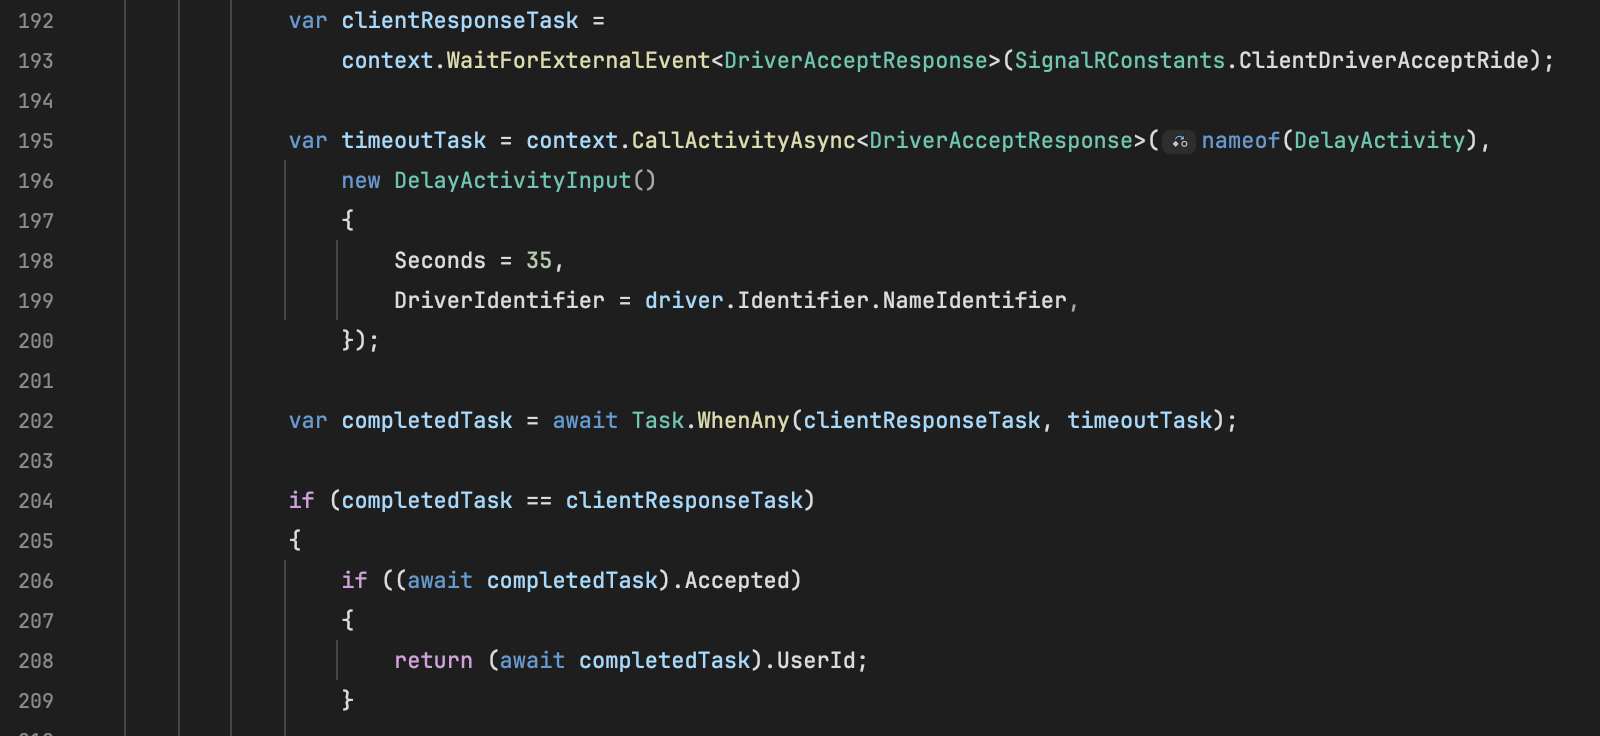
\includegraphics[width=16cm]{Assets/WaitForDriver.png}
    \caption{Așteptarea răspunsului de la șofer și cronometrarea timpului de acceptare.}
    \label{fig:WaitForDriver}
\end{figure}

La orice pas, dacă utilizatorul anulează fie confirmarea, fie plata, fie nu se găsește un șofer, cursa intră într-un status
terminal, setând proprietatea \textit{CompletedStatus} cu un status aferent acțiunii.
\begin{figure}[H]
    \centering
    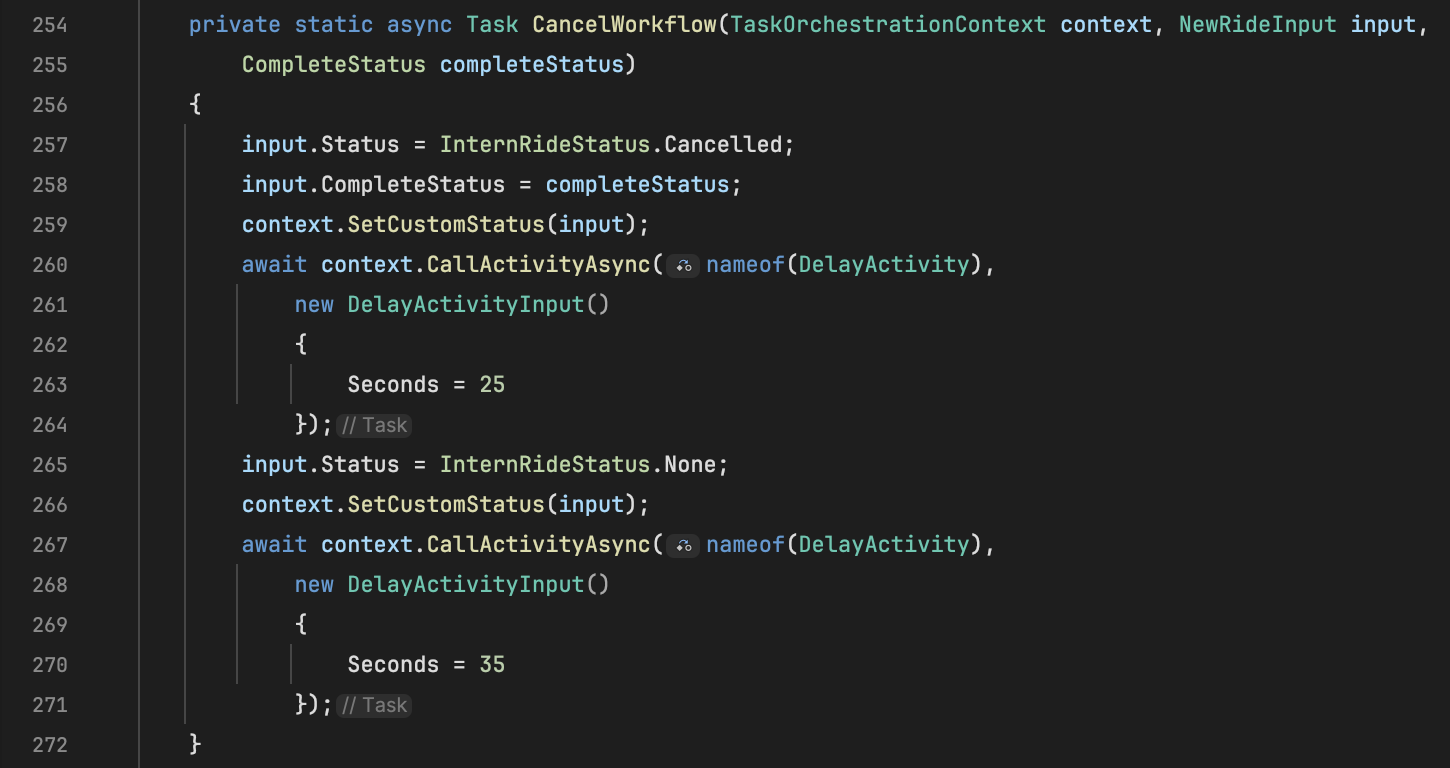
\includegraphics[width=16cm]{Assets/cancelFlow.png}
    \caption{Anularea cursei dacă plata nu s-a procesat, a fost intenționat anulată sau nu s-a găsit un șofer.}
    \label{fig:cancelFlow}
\end{figure}
Delay-urile au rolul de a face posibilă așteptarea ca și utilizatorul să primească aceste informații, altfel totul ar fi instant,
iar utlizatorul nu ar vedea niciun feedback.

Funcțiile durabile de orchestrare trebuie să fie deterministice, astfel încât dacă aplicația repornește
sau un proces de resetare intervine, codul să rezulte același rezultat. Pentru asta, trebuie evitate în contextul
orchestration-ului să se genereze valori random sau să se apeleze service-uri. Totuși, este nevoie să se apeleze service-uri precum
calcularea pretului cursei sau căutarea unui șofer. Pentru a face posibil acest lucru, intervin activtățile.

\textit{Activity functions} sunt funcții ce au rol de a menține pasul la care orchestration-ul rulează.
Pentru fiecare acțiune necesară în orchestration, există o activitate, astfel:
\begin{itemize}
    \item \textit{CancelRideActivity} - trimite cererea de anulare a cursei către toți participanții;
    \item \textit{DelayActivity} - suspendă orchestration-ul pentru \textit{n} secunde;
    \item \textit{FindDriverActivity} - caută un șofer pentru cursa trimisă. Totodată, se așteată să primească și lista de șoferi ce au fost excluși, datorită faptului că au respins deja cererea;
    \item \textit{NotifyDriverTimeoutActivity} - notifică șoferul că perioada de acceptare a cursei a expirat;
    \item \textit{SendPaymentIntentActivity} - creează \textit{PaymentIntent}-ul și îl trimite către client;
    \item \textit{SendPriceCalculationActivity} - calculează prețul cursei și îl notifică pe client despre acesta;
    \item \textit{SendRatingRequestActivity} - la finalul cursei, clienții trebuie să ofere un notă șoferului, această activitate ocupându-se de această sarcină;
    \item \textit{SendRideToDriverActivity} - notifică șoferul despre cursă, acesta fiind nevoit să decidă dacă acceptă cursa sau nu.
\end{itemize}

\begin{figure}[H]
    \centering
    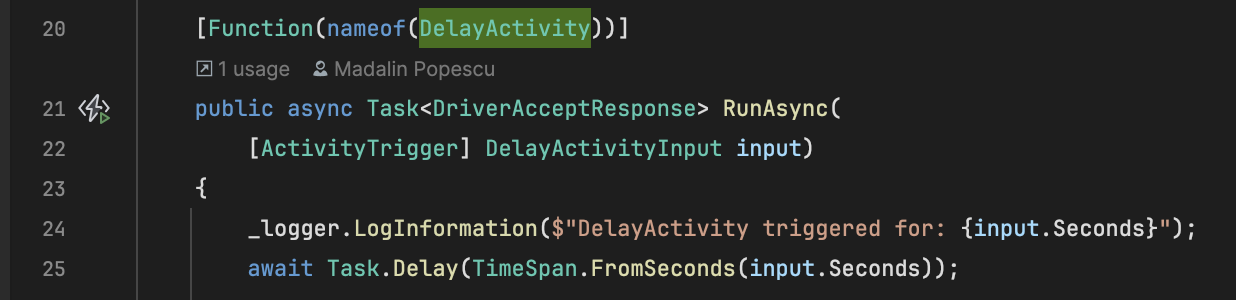
\includegraphics[width=15cm]{Assets/activities.png}
    \caption{Declararea activității ce pune orchestration-ul să aștepte \textit{n} secunde.}
    \label{fig:activities}
\end{figure}

Pentru a structura logica, separat de activități, se folosesc servicii. \textit{Services} sunt instanțe de clase înregistrate în
contextul aplicației pentru a putea fi injectate mai târziu, și folosite să execute diferită logică.
Spre exemplu, calcularea distanței dintre două puncte este o metodă dintr-un service înregistrat \textit{Scoped} (se generează o instanță nouă
la fiecare request inițiat). Alte servicii ce se regăsesc în proiect sunt pentru calcularea prețului, pentru
a găsi șoferi în zonă apropiată de un client și de a intermedia operațiile \textit{CRUD} (Create Read Update Delete) pentru utilizatori și curse.
Toate serviciile folosesc o structură comună de returnare a datelor, răspunsul fiind încapsulat într-un \textit{ServiceResponse}
ce conține payload-ul, un mesaj de eroare sau o excepție, dacă există și dacă totul s-a executat cu succes sau nu. Acest tip de răspuns
ajută la handle-uirea răspunsului și încapsularea lui într-un \textit{ApiResponse}.

Configurarea proiectului se face prin \textit{Environment Variables}, local, definindu-se prin
\textit{local.settings.json}. Această configurație este alcătuită din:
\begin{itemize}
    \item Google Credentials - pentru a reuși validarea token-ului de acces ce vine pe request;
    \item Distance Configuration - ce conțin prețurile pentru un kilometru, un minut, prețul inițial și viteza medie de calcul pentru distanță;
    \item Stripe Secret Key - folosit pentru generarea intenționării de plată;
    \item Storage Connection String - conexiunea la Azure Storage.
    \item SignalR Connection String - conexiunea la server-ul SignalR
\end{itemize}

Microsoft, loghează fiecare activitate ce se execută, iar în caz de deployment pe o infrastructură ce permite logging (spre exemplu Azure),
este necesar să se specifice ce anume să se logheze pentru a nu se ajunge la costuri mari
\begin{figure}[H]
    \centering
    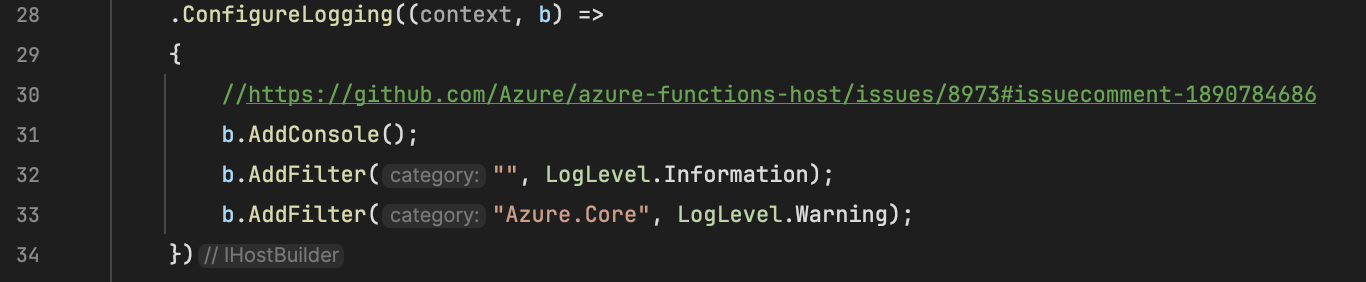
\includegraphics[width=16cm]{Assets/configLogging.png}
    \caption{Filtrarea log-urilor din Azure.}
    \label{fig:configLogging}
\end{figure}

\subsection{Client-side}

Client-side-ul se ocupă cu afișarea informațiilor procesate pe Server. La bază, stă
Blazor WASM, ce funcționează fără a avea nevoie de o componentă de server sau să instanțieze
două componente de comunicare. Toate asset-urile se descarcă în browserul utilizatorului și poate funcționa fără conexiune la internet.

Folderul \textit{wwwroot} este rădăcina conținutului static al aplicației Blazor WebAssembly.
Tot ce se află în acest folder (sau în subfolderele lui) este expus publicului și servit direct browserului, fără procesare pe server.
Aici se regăseștex configurația proiectului pentru debugging, stilurile CSS, logica JavaScript, dar și datele mock pentru debugging.

\begin{figure}[H]
    \centering
    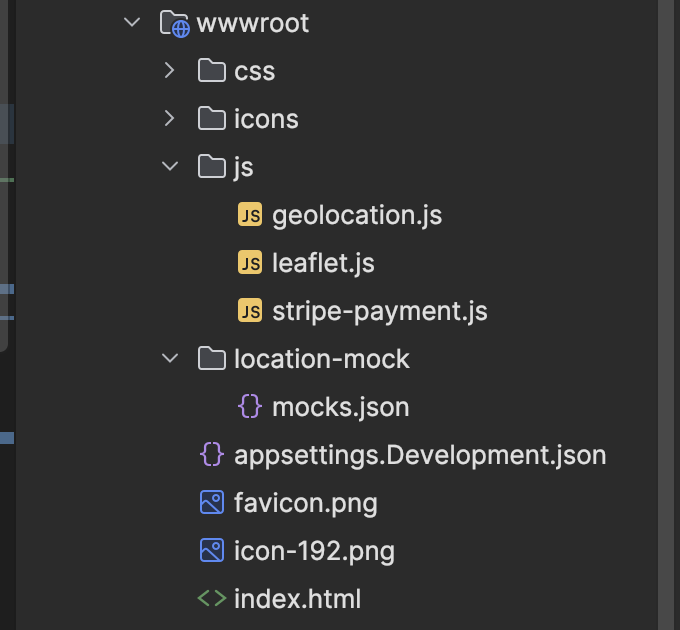
\includegraphics[width=10cm]{Assets/wwwroot.png}
    \caption{Conținutul folderului \textit{wwwwroot}.}
    \label{fig:wwwroot}
\end{figure}

\textit{Configurația proiectului} conține informațiile de autentificare pentru Google (\textit{ClientId}, \textit{Authority}, \textit{Scopes}, etc),
setări predefinite pentru hartă, conexiunea cu server-ul și \textit{PublishKey}-ul pentru Stripe.

Sistemul de hărți este susținut de Leaflet, combinat cu modulul Routing Machine pentru calcularea traseului.
Există un Nuget Package pentru Blazor însă suportul pentru Routing nu vine inclus. De aceea se folosește librăria așa
cum vine ea, fără alte pachete instalate, doar prin JavaScript.

Pentru a face legătura dintre Blazor (C\#) și JavaScript, există JSInterop. \textit{JSInterop}
(JavaScript Interop) este mecanismul prin care aplicațiile Blazor pot comunica cu
JavaScript. Prin JSInterop, codul scris în C\# poate apela funcții JavaScript, iar
JavaScript poate la rândul său să invoce metode din C\#. Acest mecanism este esențial
atunci când Blazor nu oferă suport direct pentru anumite funcționalități disponibile
doar prin API-urile browserului sau prin biblioteci JavaScript externe. Interacțiunea
este asincronă și se realizează prin intermediul interfeței \textit{IJSRuntime}, fiind
disponibilă atât în Blazor WebAssembly, cât și în Blazor Server. \parencite{blazor}

Urmând pașii de folosire a hărții Leaflet, s-a creat un script în JS, pentru a putea fi
apelat din Blazor și a inițializa harta. Totul s-a încapsulat într-o componentă \textit{Map.razor}.
După ce componenta se randează, se construiește harta, care suprascrie un \textit{div} tag cu ID-ul \textit{map}, instanțiază
un \textit{.NET Object Reference} (pentru a putea fi apelat codul .NET din JS) și se folosește de informațiile despre locația curentă, zoom-ul
pe hartă și alte setări pentru configurare.

\begin{figure}[H]
    \centering
    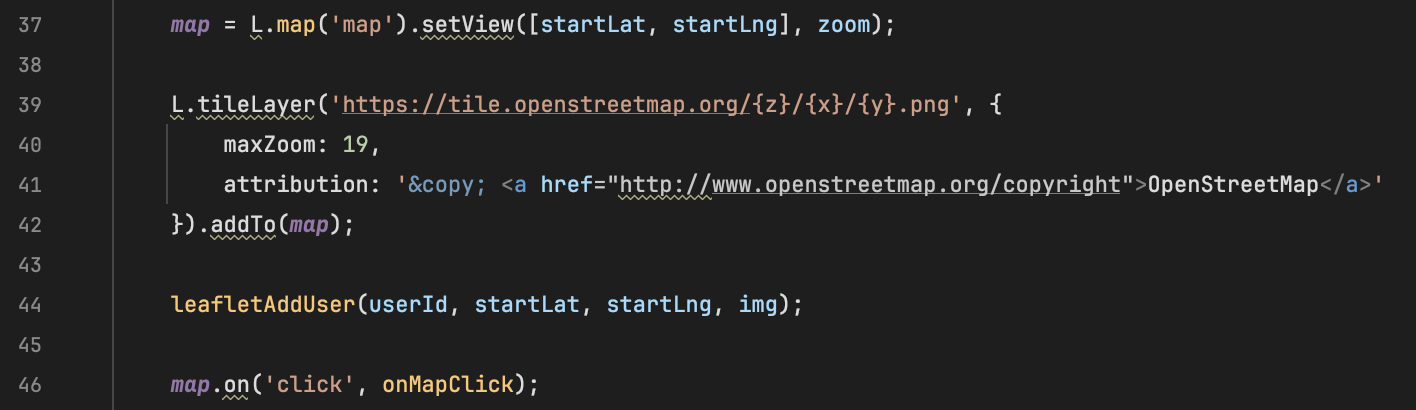
\includegraphics[width=16cm]{Assets/initLeaflet.png}
    \caption{Inițializarea hărții după ce componenta s-a randat.}
    \label{fig:initLeaflet}
\end{figure}

Orice iconiță adăugată pe hartă reprezintă un \textit{marker} cu o imagine ca și înfățișare. Pentru a pune un \textit{pin}, spre exemplu, există o metodă numită \textit{SetPinLocationAsync} ce adaugă un \textit{marker} pe hartă cu \textit{asset-ul de pin}.
Toate asset-urile se află în \textit{wwwwroot/icons}: \textit{pin}, \textit{human}, \textit{driver} și \textit{currentCar} (ce indică că atât clientul cât și șoferul se află în aceiași mașină).
Metodele \textit{DrawRoute} și \textit{AddUser/Driver} ajută la construirea traseului și adăugarea unui utilizator pe hartă.

\begin{figure}[H]
    \centering
    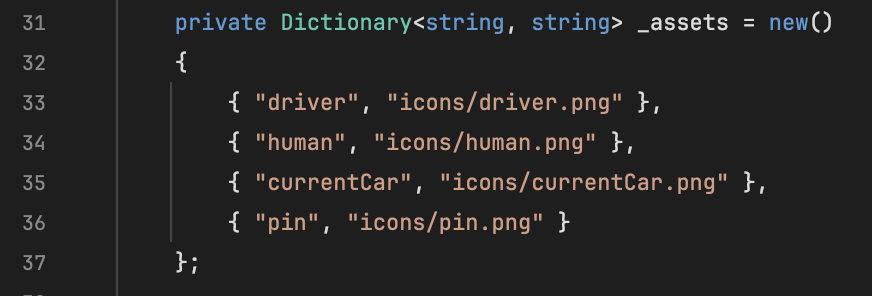
\includegraphics[width=14cm]{Assets/icons.png}
    \caption{Dicționarul ce face legătura dintre tipul de marker și imaginea de îl reprezintă.}
    \label{fig:icons}
\end{figure}

Același mecanism de afișare îl folosește și dialog-ul pentru a introduce cardul bancar.
Se atașează input-urile de elementul \textit{div} cu ID-ul \textit{payment-element}. Acesta
validează un card bancar folosind API-ul Stripe, iar pentru a putea autoriza acest request,
se folosește de \textit{PublishKey} din dashboard-ul Stripe.

\begin{figure}[H]
    \centering
    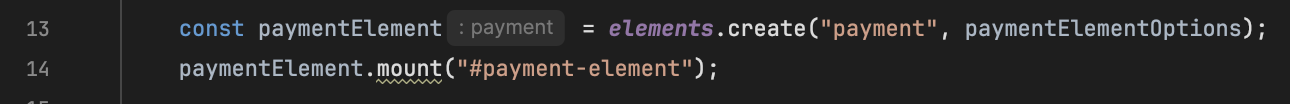
\includegraphics[width=16cm]{Assets/stripeMount.png}
    \caption{Atașarea input-ului pentru card bancar de elementul cu ID-ul \textit{payment-element}.}
    \label{fig:stripeMount}
\end{figure}

Toate tranzacțiile sunt se pot vedea în platfomă, dacă au fost cu succes, ce card a fost folosit sau de către ce customer a fost plătit.
Fiind în modul de testare, se poate folosi doar cardul cu numărul: \textit{4242 4242 4242 4242}, restul informațiilor
trebuind să fie doar corecte, nu și existente.

\begin{figure}[H]
    \centering
    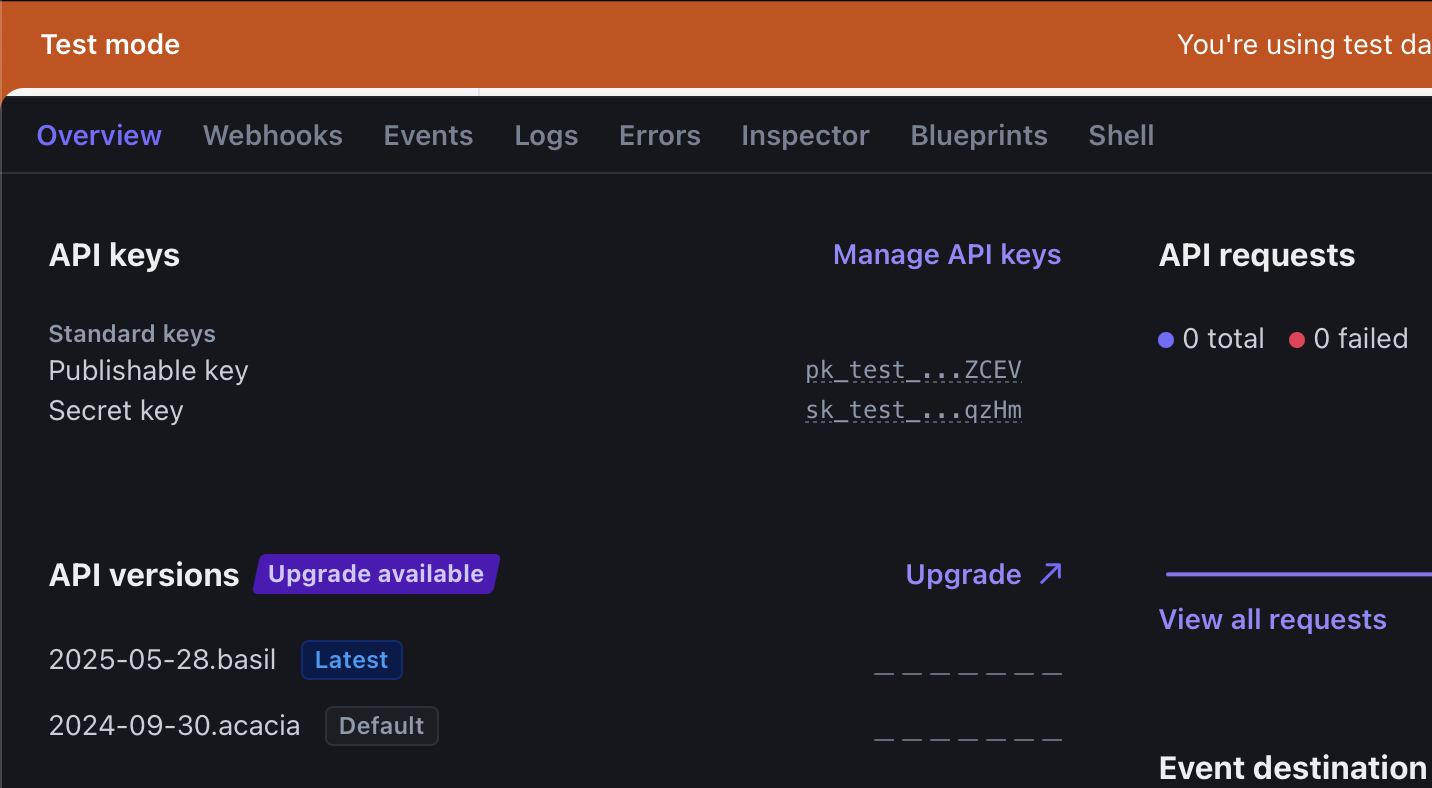
\includegraphics[width=14cm]{Assets/stripeSite.png}
    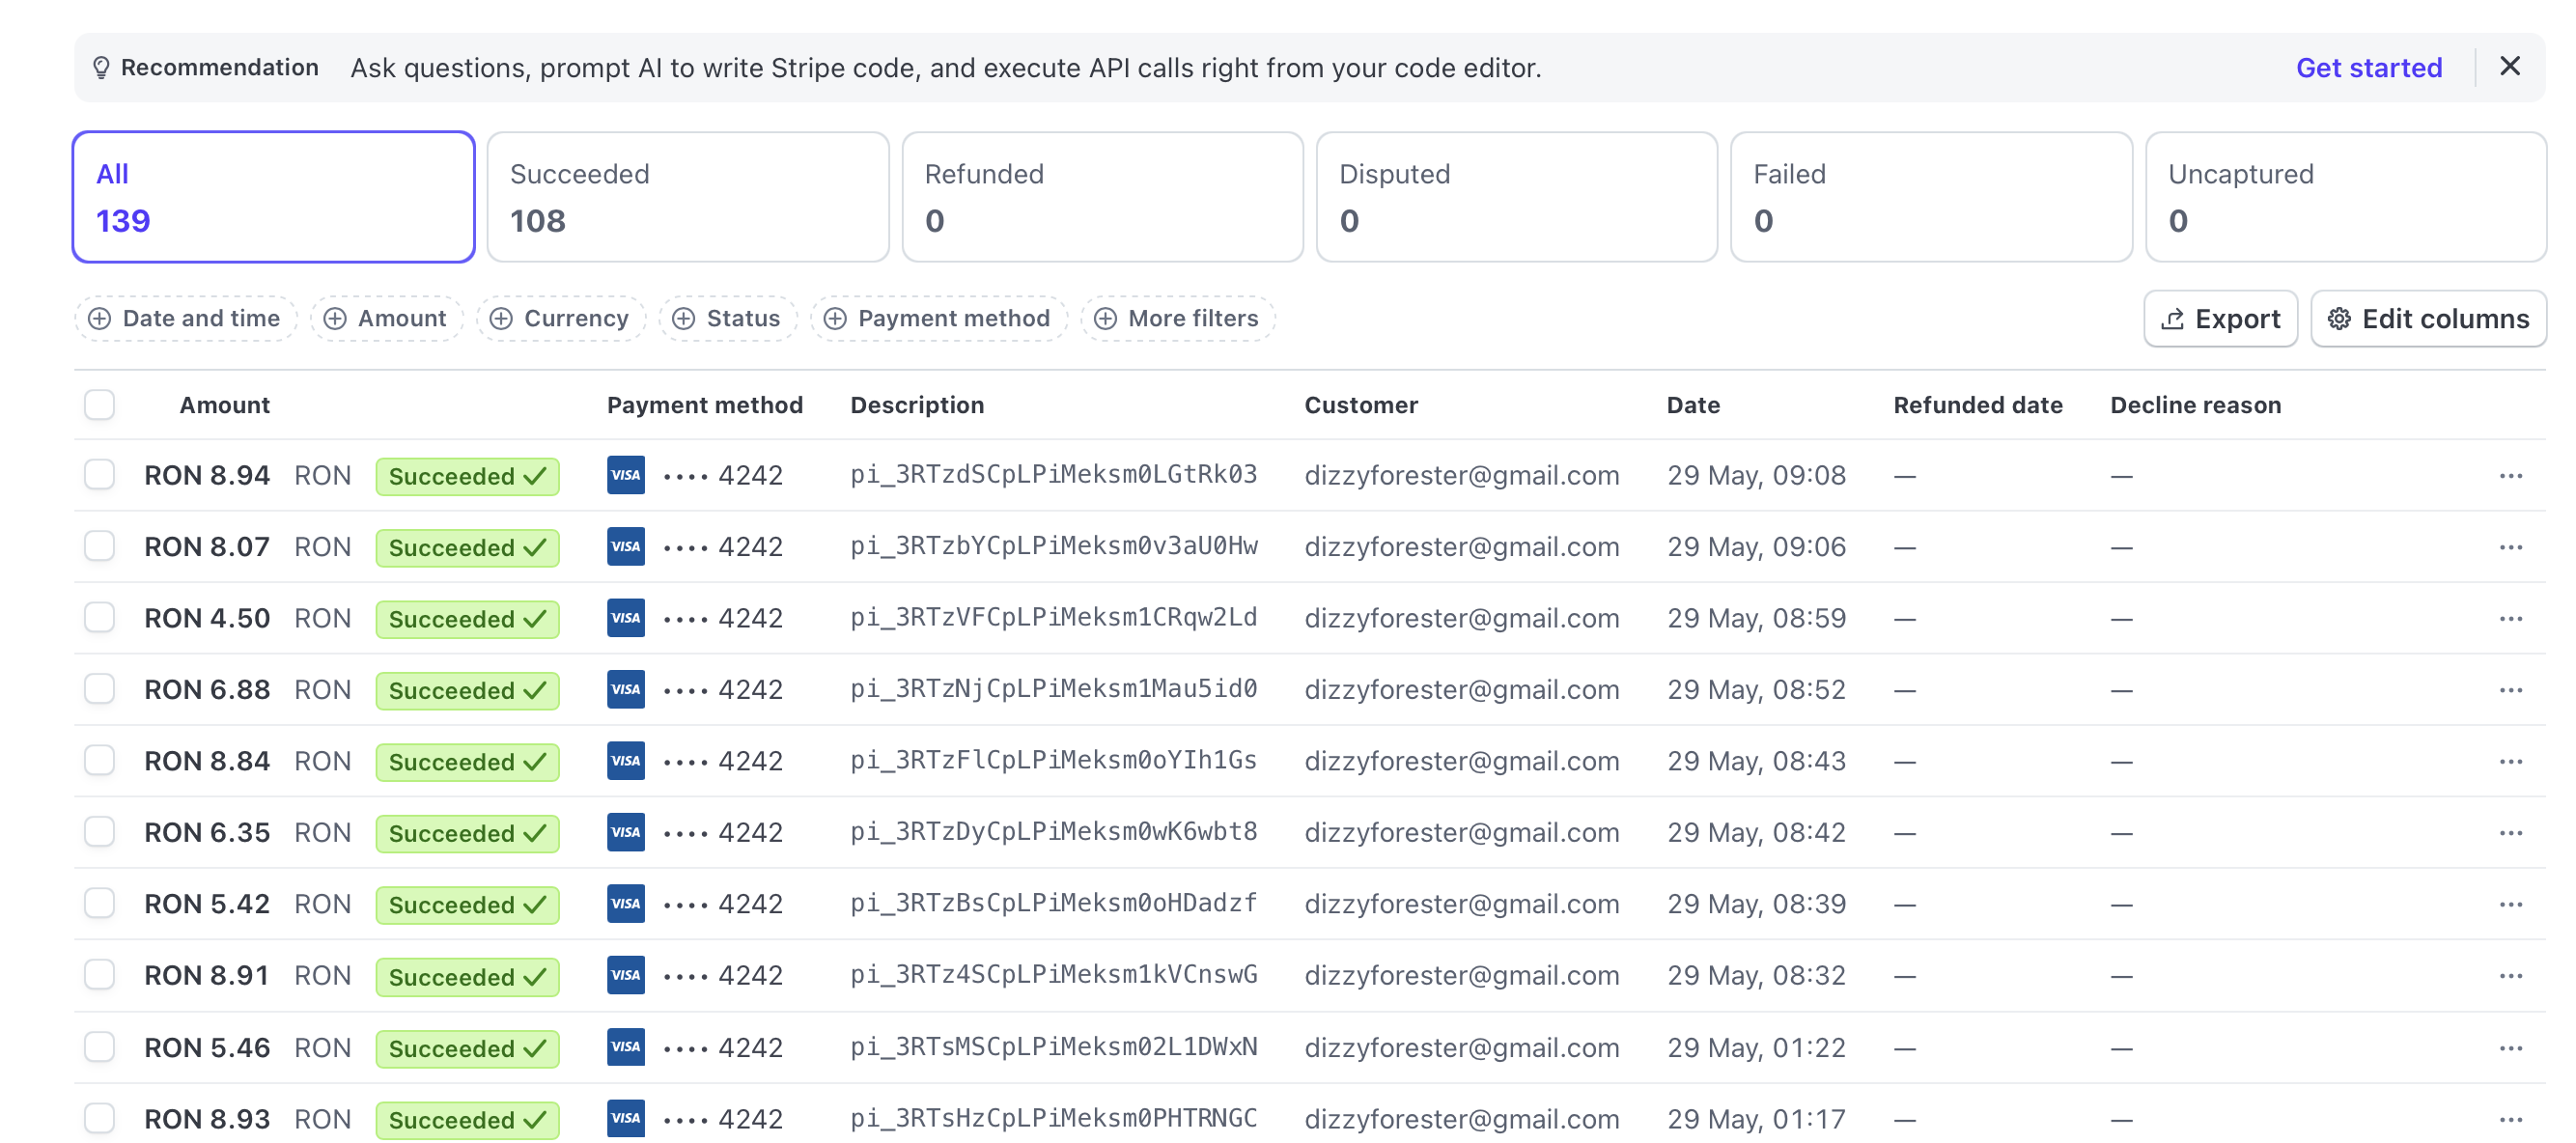
\includegraphics[width=14cm]{Assets/stripeHistory.png}
    \caption{Configurarea Stripe în dashboard-ul platformei și istoricul tranzacțiilor.}
    \label{fig:stripeSiteHistory}
\end{figure}

Pentru transmiterea live a locației curente de către utilizatori și de a reuși să se expună pe hartă
locul exact unde se află utilizatorul, se folosește un \textit{Background Service} ce rulează în constant și face request de locație către JavaScript.
Background Service-ul face acest tip de request din trei în trei secunde, folosind un \textit{PeriodicTimer}.

\begin{figure}[H]
    \centering
    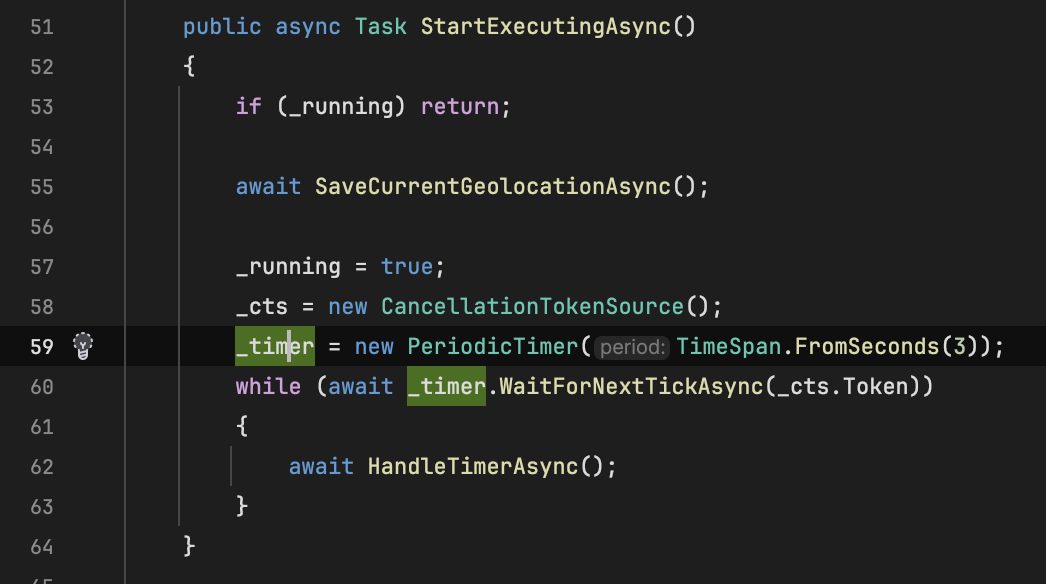
\includegraphics[width=14cm]{Assets/timer.png}
    \caption{Execuția din 3 în 3 secunde a Backgroud Service-ului.}
    \label{fig:timer}
\end{figure}

Pentru a reuși să se obțină locația curentă, codul din JavaScript nu returnează instant rezultatul, ci
apelează un \textit{callback method}. Astfel, pentru a reuși să se aștepte acest răspuns în .NET, se folosește
\textit{TaskCompletionSource} ce asteaptă pentru un \textit{event}, mai exact ca acesta să își schimbe state-ul și
să i se seteze un rezultat.

\begin{figure}[H]
    \centering
    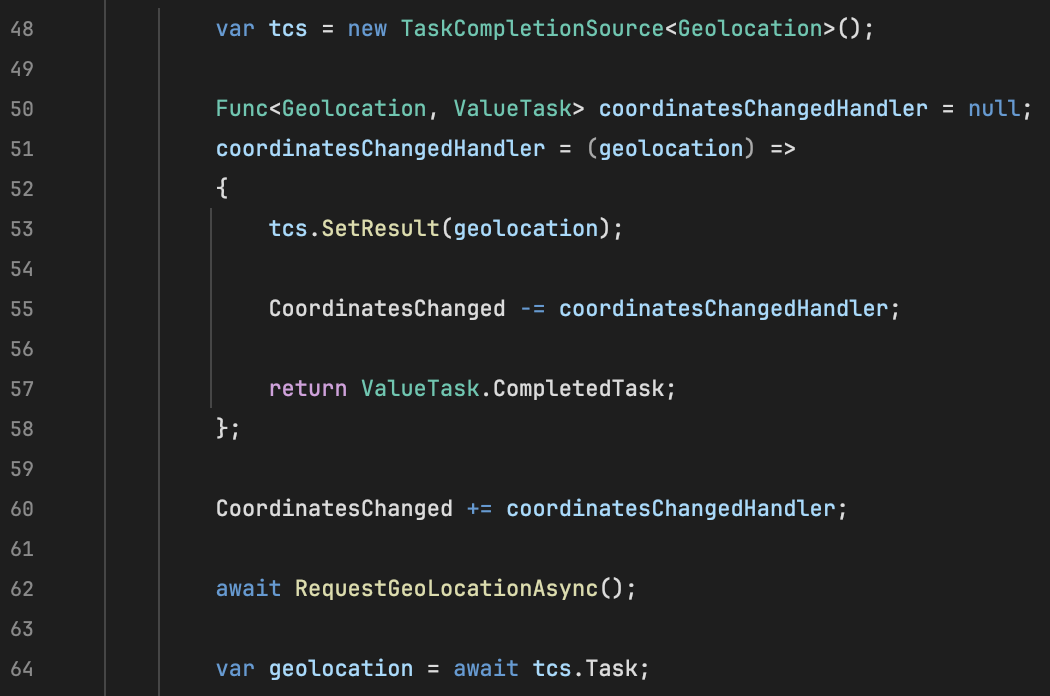
\includegraphics[width=14cm]{Assets/tcs.png}
    \caption{\textit{TaskCompletionSource} asteptând ca scriptul de JavaScript să trigger-uiască event-ul \textit{CoordinatesChanged}}
    \label{fig:tcs}
\end{figure}

Pentru reuși să se păstreze acest tip de informații (locația curentă, status-ul curent al cursei,
grupul din care face parte utilizatorul) se folosesc \textit{State}-urile. Un \textit{State} este un service
care nu necesită o interfață deoarece nu este făcut să handle-uiască logică, ci doar să
păstreze valoarea unor proprietăți pe parcursul execuției. Ele se înregistreză \textit{Scoped}
pentru a se reseta instanța în momentul unui request nou (adică dacă alt utilizator deschide site-ul sau dă refresh), astfel
valorile unui utilizator nu o să interfereze cu ale celorlalți.

Grupul din care face parte utilizatorul, despre care s-a menționat în secțiune de Server, se calculează
aici deoarece Client-ul este singurul loc unde se poate detecta locația utilizatorului.
Grupul este format din oraș, județ și țară și se poate află folosind service-ul \textit{IUserGroupService}.
Dacă utilizatorul se află într-o cursă, atunci service-ul returnează ID-ul cursei ca și grup pentru a reuși să
se facă o conexiune doar între client și șofer.

Pentru informații precum: detectarea adresei în text, folosind geolocația, se folosește service-ul
\textit{ILocationService} ce folosește API-ul de la \textit{OpenStreetMap}.

Pe lângă componenta hărții, mai există componentele ce implementează dialog-urile pentru
rating, acceptarea cursei, plătirea cursei și componente precum \textit{loading screen}-ul,
afișarea status-ului cursei (dacă este există una în progres) și butoane (pentru a porni o cursă sau a deschide dialog-ul de permite acceptarea uneia).

Pagina principală conține harta, un search pentru adrese, ce interoghează API-ul de la \textit{OpenStreetMap}
cu query-ul introdus de utilizator și returnează o listă de sugestii.

Pagina \textit{History} conține
istoricul curselor cu informații despre cursă precum prețul, data, dar și locația.

Adminii beneficiază de o pagină în plus
unde pot vedea toți utilizatorii și le pot modifica informații precum numărul de telefon sau rolul.

Infomațiile precum, numele sau imaginea sunt informații ce vin de pe contul Google al utilizatorului și acesta
este redirecționat către pagina Google Accounts pentru a putea actualiza ce dorește. Toate acestea reprezentând și butoanele \textit{nav-menu}-ului.

Autentificarea se face prin Google, astfel utilizatorul, dacă nu este autentificat, este redirecționat către
pagina de autentificare ce face un \textit{remote authentication}.

\begin{figure}[H]
    \centering
    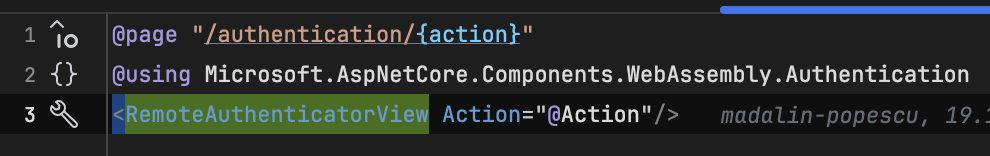
\includegraphics[width=14cm]{Assets/authenticationRemote.png}
    \caption{Pagina de autentificare ce redirecționeză utilizatorul către Google Login.}
    \label{fig:authenticationRemote}
\end{figure}

Pentru a putea autoriza butoane sau pagini, se folosește atributul \textit{Authorize}. Acesta se folosește de
un \textit{AccountClaimsPrincipalFactory} și un \textit{RemoteUserAccount} pentru a știi ce roluri se află pe token-ul utilizatorului.

\begin{figure}[H]
    \centering
    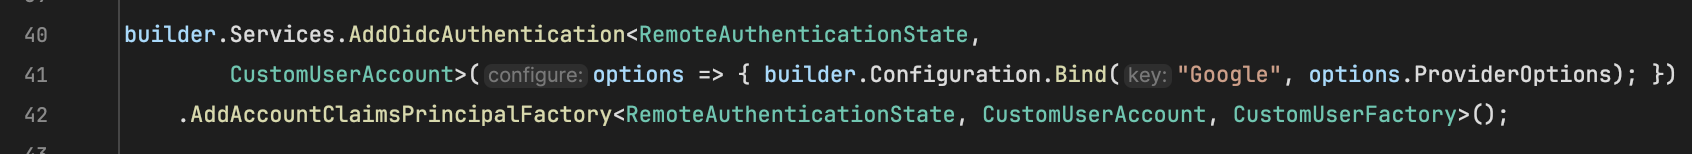
\includegraphics[width=16cm]{Assets/registerAuthentication.png}
    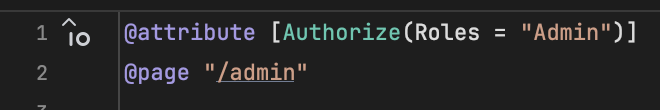
\includegraphics[width=8cm]{Assets/authorizeAttribute.png}
    \caption{Înregistrarea autenficării și folosirea autorizării în aplicație.}
    \label{fig:registerUseAuth}
\end{figure}

Layout-ul aplicației este cuprins dintr-un \textit{navigation bar}, dialog-ul ce afișează status-ul cursei curente, loading screen-ul
ce ascultă la State-ul \textit{OverlayState},dar și content-ul propriu zis al paginii curente.

Testarea unui asemenea proiect este dificil deoarece nimeni nu își dorește să se plimbe prin oraș pentru a îndeplini \textit{test-case}-urile.
Schimbarea locației unui dispozitiv fără un VPN este dificilă deoarece trebuie "păcălit" mai întâi browser-ul și apoi codul.
De aceea, se folosesc date de testare, mock-uite, astfel utilizatorii cu un anumit identificator pot fi localizați în locuri
diferite datorită fișierului \textit{mocks.json}.

\begin{figure}[H]
    \centering
    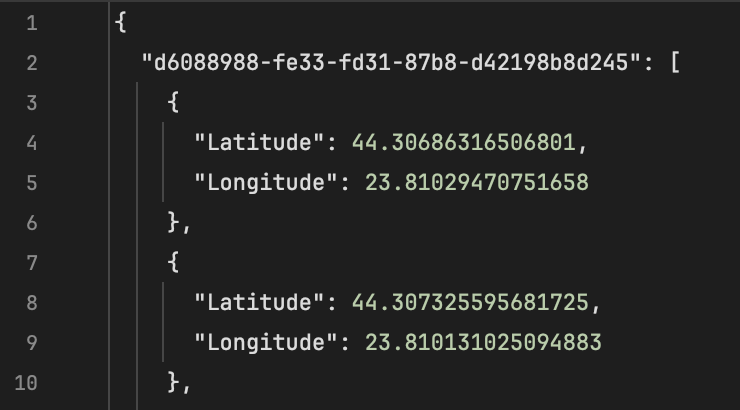
\includegraphics[width=14cm]{Assets/dynamicMocks.png}
    \caption{Fișiserul JSON ce conține coordonatele mock-uite pentru utilizatori.}
    \label{fig:dynamicMocks}
\end{figure}

Aceste date sunt preluate de către Background Service la fiecare trei secunde și sunt parcurse una câte una.
În plus, metoda \textit{HandleGeolocationMockAsync} interacționează cu datele acestui fișier pentru a putea
face posibila staționarea utilizatorilor sau resetarea index-ului de iterație prin fișier.

Pentru lucrarea curentă, s-a pregătit un singur set de date, astfel punctul de plecare se află
pe Strada Anului 1848, Craiova, iar punctul de sosire este pe Strada Târgului, Craiova.

\section{Comunicarea între componente}

\begin{figure}[H]
    \centering
    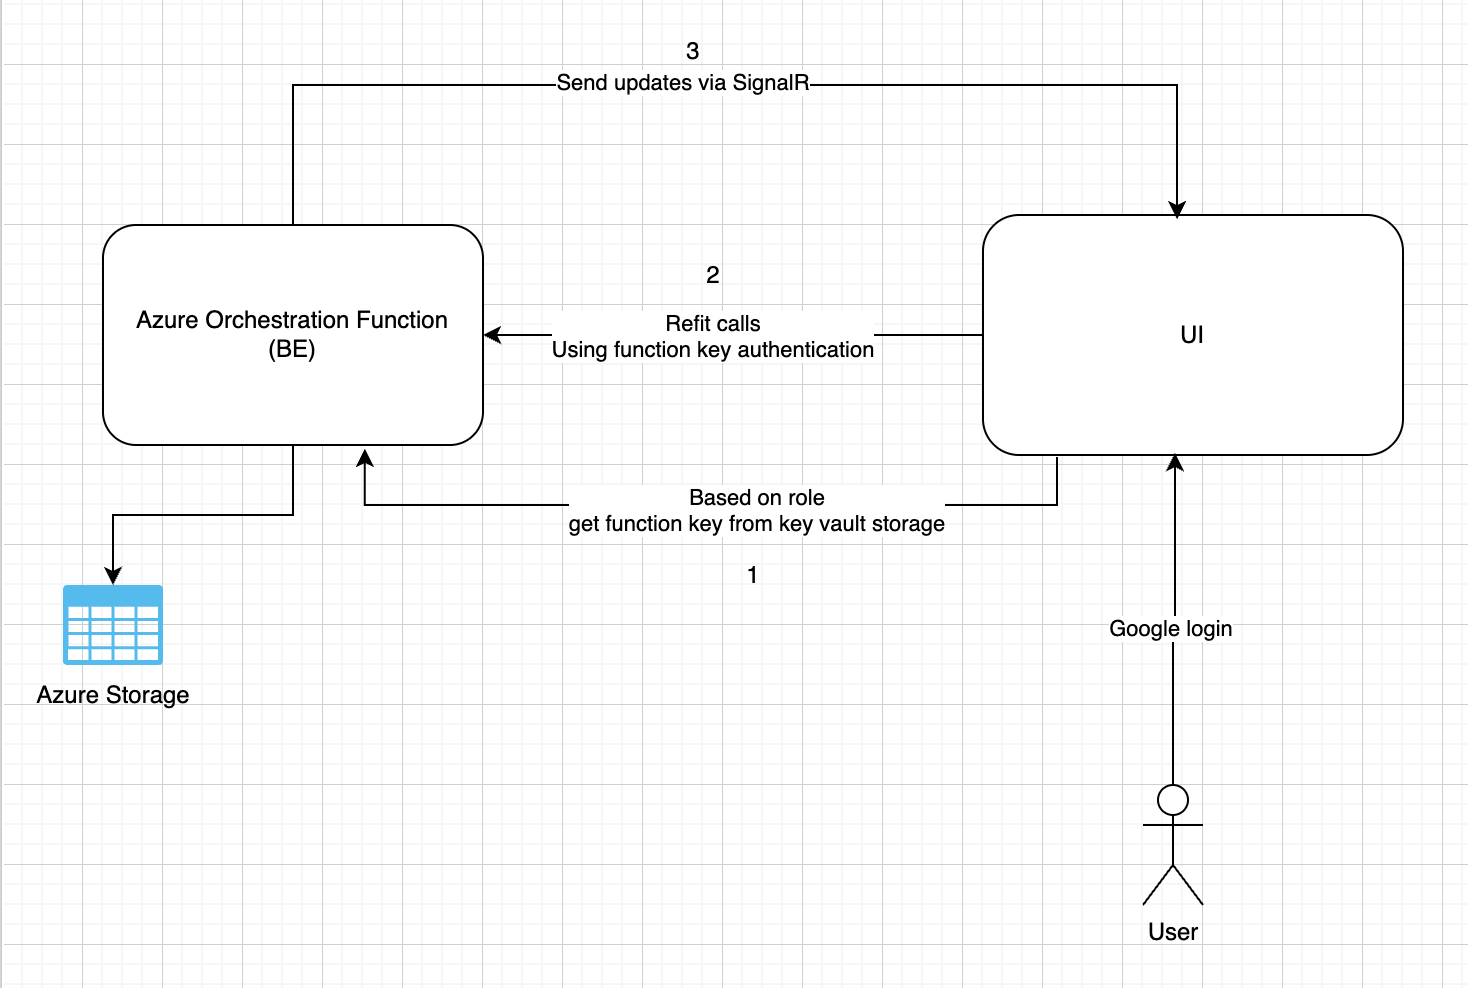
\includegraphics[width=16cm]{Assets/componentsComunication.png}
    \caption{Comunicarea dintre componentele proiectului.}
    \label{fig:componentsComunication}
\end{figure}

Componentele proiectului comunică în perechi de câte două: Server-ul fiind
cel ce gestionează atât Client-ul cât și Storage-ul.

Comunicarea cu Client-ul se face prin două căi: HTTP request și SignalR.

Comunicarea prin request-uri HTTP, se realizează prin librăria \textit{Refit} ce permite
serializarea și deserializarea request-ului și response-ului într-un mod mult mai ușor de folosit,
apelarea și autorizarea endpoint-urilor de pe backend fără a fi nevoie de crearea unui \textit{HttpClient}
și configurarea acestuia. Librăria doar face public un contract astfel încât, celelalte aplicații pot folosi doar ce li se dispune.
Pentru acest lucru, s-a creat un proiect comun între cele două componente, numit \textit{SDK}.
Acesta poate fi folosit și ca \textit{NuGet Package} pentru separarea soluțiilor în repository-uri diferite.

Proiectul se folosește de o clasă abstractă intermediară și un client ce customizează interfața Refit,
pentru a reuși să aducă toate response-urile într-un anumit format (\textit{ApiResponseMessage}).

\begin{figure}[H]
    \centering
    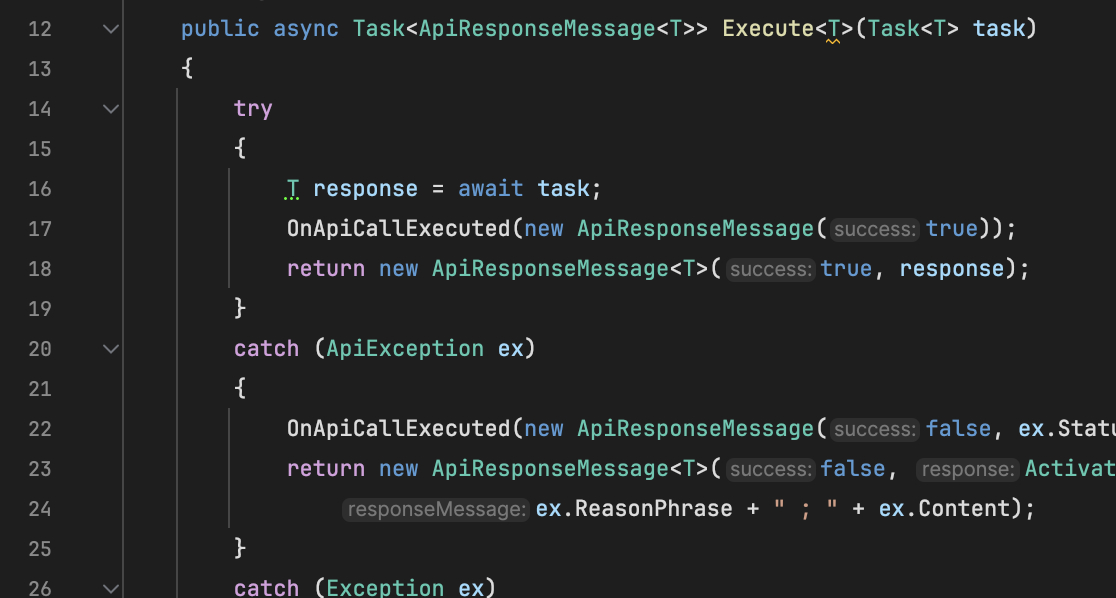
\includegraphics[width=14cm]{Assets/refitAbstract.png}
    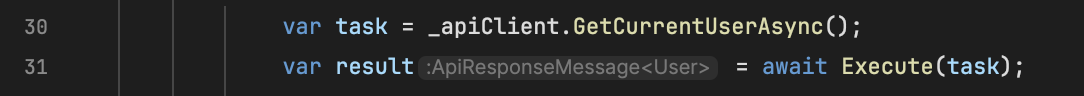
\includegraphics[width=14cm]{Assets/userRefitAbstract.png}
    \caption{Metoda ce obține rezultatul dorit în urma execuției endpoint-ului.}
    \label{fig:refitAbstract}
\end{figure}

Refit are nevoie doar de o interfață pentru a reuși să inițieze request-ul, unde trebuie să se specifice ruta, tipul request-ului și eventuali parametri
împreună cu tipul răspunsului.

\begin{figure}[H]
    \centering
    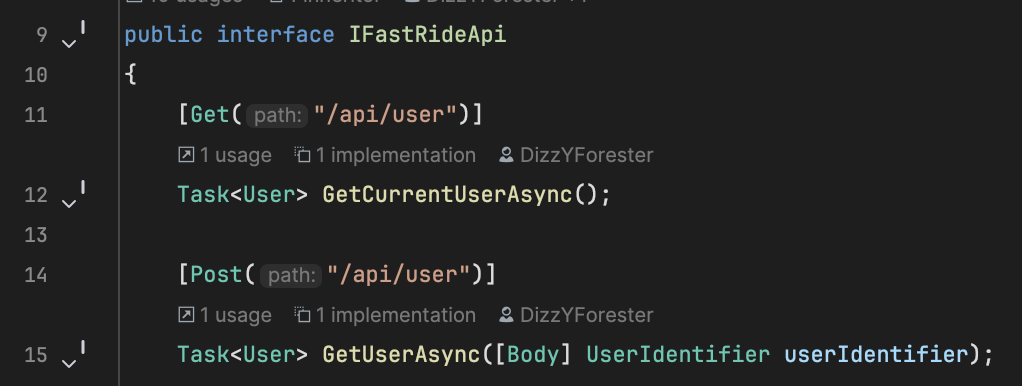
\includegraphics[width=14cm]{Assets/refitInterface.png}
    \caption{Interfața Refit.}
    \label{fig:refitInterface}
\end{figure}

Pentru a autoriza orice request, Client-ul trebuie să ofere o implemetare pentru un \textit{DelegatingHandler}, ce 
are rolul să interferează, ca un interceptor, la orice request făcut din interiorul host-ului și să adauge
pe request \textit{Authorization headers}.

\begin{figure}[H]
    \centering
    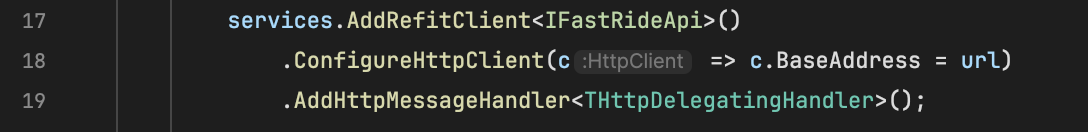
\includegraphics[width=15cm]{Assets/configureDelegate1.png}
    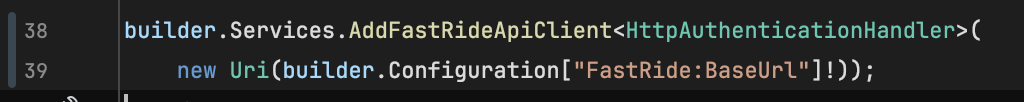
\includegraphics[width=15cm]{Assets/configureDelegate2.png}
    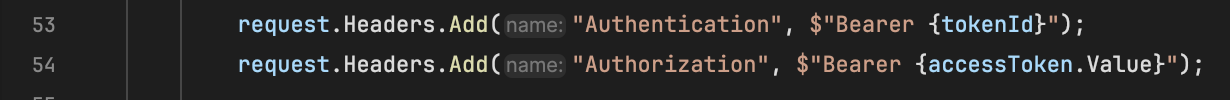
\includegraphics[width=16cm]{Assets/configureDelegate3.png}
    \caption{Înregistrarea DelegatingHandler-ului din Client (\textit{THttpDelegatingHandler} este \textit{HttpAuhenticationHandler})
        și adăugarea header-urilor de autentificare și autorizare.}
    \label{fig:configureDelegate}
\end{figure}

Comunicarea prin SignalR se realizează fără un intermediar. Server-ul tratează mesajele de intrare și de ieșire folosind
\textit{Functions}, așa cum s-a arătat în descrierea componentei Server.

Pe partea de client, toate aceste mesaje se tratează folosind un serviciu. Astfel, se instanțiază
o conexiune cu server-ul SignalR și se crează subscripții pentru mesajele de pe Server.
Fiecare subscripție notifică un \textit{event} din serviciu, care este, mai departe, ascultat de componente pentru
a putea actualiza interfața.

\begin{figure}[H]
    \centering
    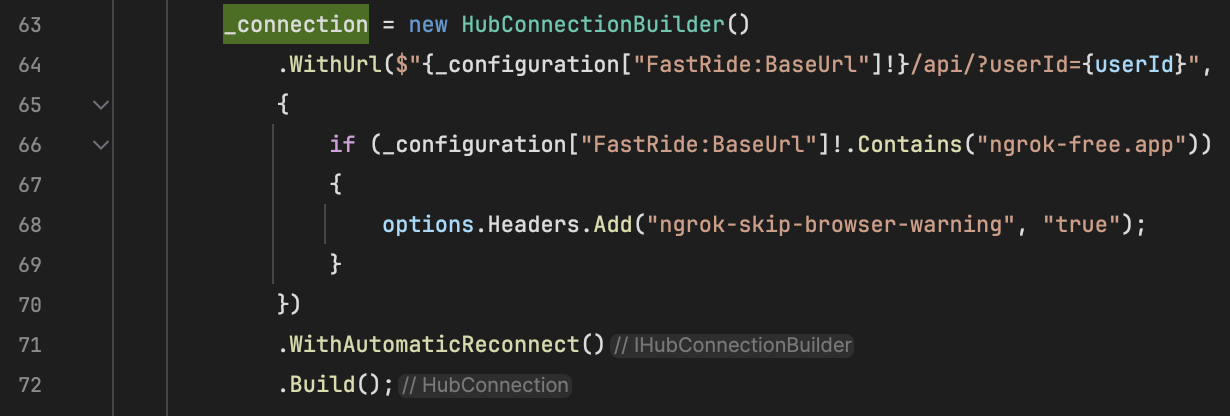
\includegraphics[width=16cm]{Assets/signalrConnect.png}
    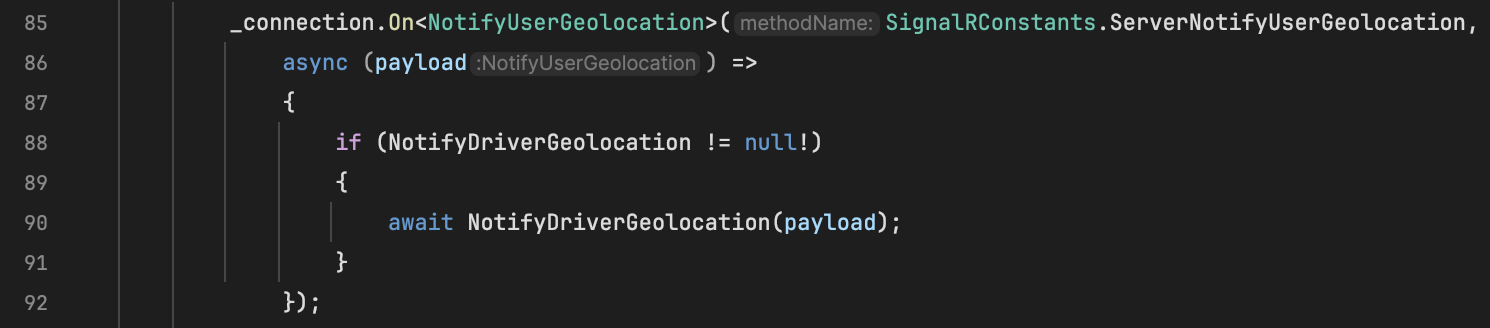
\includegraphics[width=16cm]{Assets/signalROn.png}
    \caption{Conectarea la server-ul SignalR și crearea subscripției pentru notificarea noii locații a unui șofer pe hartă.}
    \label{fig:signalR}
\end{figure}

Pentru a trimite mesaje către Server (adică un alt utilizator) trebuie doar să se specifice numele evenimentului
și să se pună în ordine parametrii pe care îi așteaptă Server-ul.

\begin{figure}[H]
    \centering
    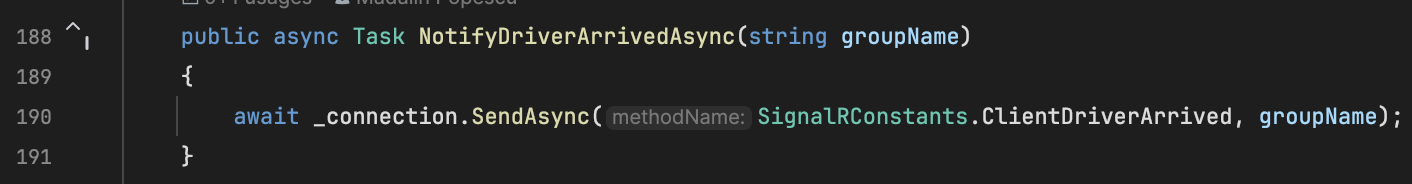
\includegraphics[width=16cm]{Assets/signalrSend.png}
    \caption{Trimiterea notificării către utilizator că s-a ajuns la unul din checkpoint-uri.}
    \label{fig:signalRSend}
\end{figure}

Pentru a știi ce tipuri de evenimete se folosesc, în proiectul de contracte pentru Refit s-a adăugat și o clasă
de constante ce conține toate evenimentele existente în aplicație. Acestea au o format comun:
\textit{\{source\}.\{action\}}. Spre exemplu \textit{client.join-user-group} este compus din sursa \textit{client} ce semnifică faptul că
mesajul este trimis de pe Client pe Server și acțiunea \textit{join-user-group} ce reprezintă cererea de a înscrie un utilizator în grupul ce se trimite ca parametru.

Comunicarea dintre Server și storage se face folosind \textit{Repository pattern}. Implentările conțin un client
ce comunică cu Azure Storage. Acest client este o interfață \textit{ITableClient<TEntity>} ce suportă
metode de GET, ADD/UPDATE și DELETE. Pentru acestea, se folosește \textit{TableClient} din Azure ce face HTTP request-uri
către Azure Storage pentru a îndeplini acțiunile dorite.

Pentru ca Azure să recunoască modelele ce reprezintă entități, acestea trebuie să implementeze interfața
\textit{ITableEntity} ce conține cheile primare (\textit{PartitionKey} și \textit{RowKey}).

Pentru a oferi un nume tabelului, s-a creat un atribut ce poate fi folosit pe toate entitățile:

\begin{figure}[H]
    \centering
    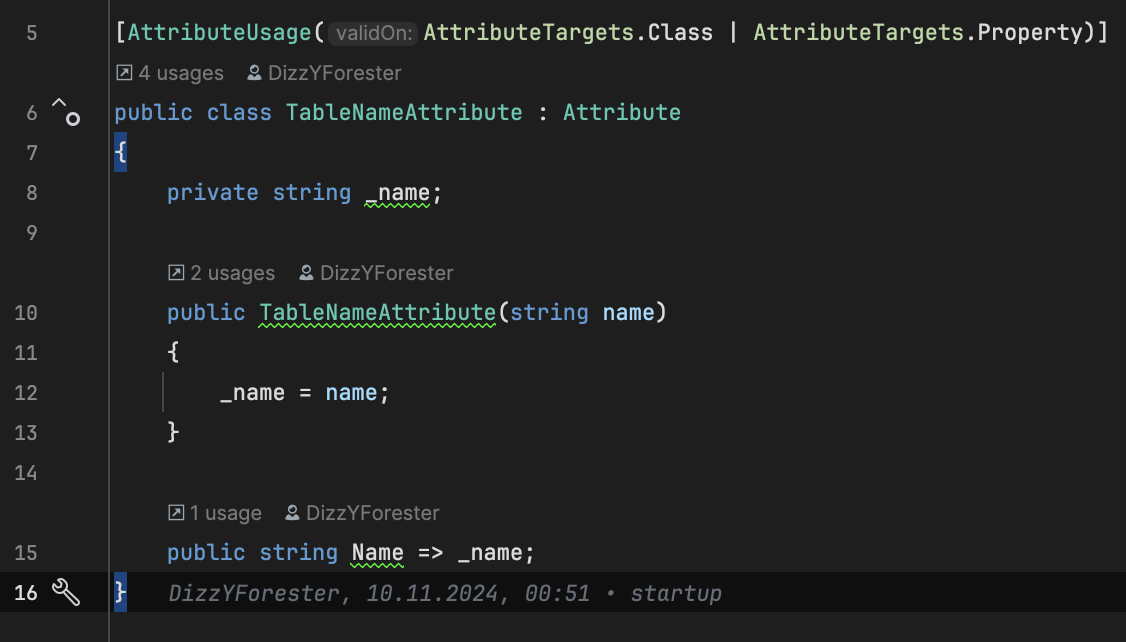
\includegraphics[width=16cm]{Assets/tableAttribute.png}
    \caption{Atributul ce atribuie entități un nume de tabel pentru storage}
    \label{fig:tableAttribute}
\end{figure}

\begin{figure}[H]
    \centering
    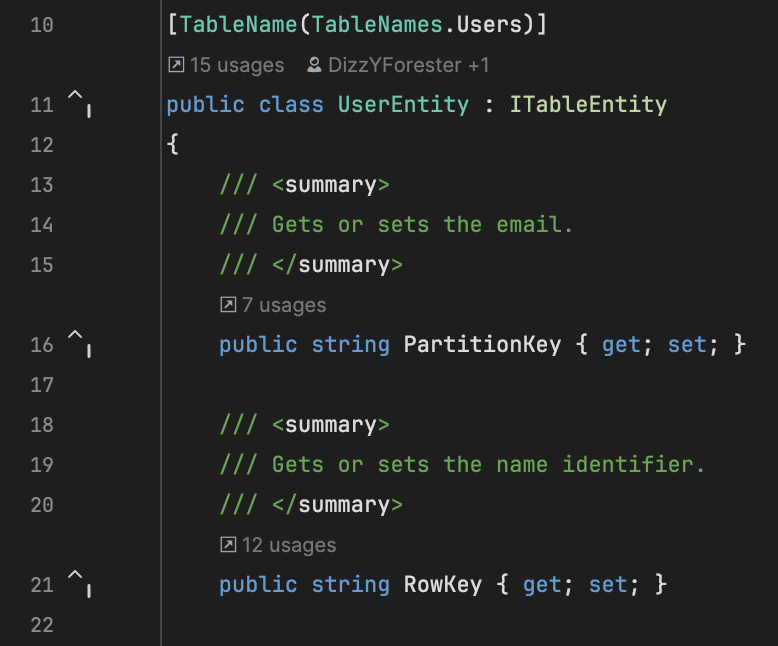
\includegraphics[width=14cm]{Assets/userEntity.png}
    \caption{Cum se folosește atributul \textit{TableName} pe entitatea \textit{userEntity}.}
    \label{fig:userEntity}
\end{figure}
